\documentclass{article}
\usepackage{graphicx} % Required for inserting images
\usepackage{listings}
\usepackage{xcolor}
\usepackage{amsmath}
\usepackage{amssymb}     % Necesario para símbolos matemáticos avanzados
\usepackage[ruled,vlined]{algorithm2e} % Necesario para el entorno \begin{algorithm} y sus comandos (\SetKwProg, \KwRet, etc.)
\usepackage{booktabs}    % Recomendado para mejorar la apariencia de las tablas


\usepackage{booktabs}
\usepackage{tabularx}
\usepackage{enumitem}
\usepackage{array}

\title{Proyecto sistemas complejos}
\author{
Juan Pablo Bustos \\
Juan Esteban Martinez \\
David Esteban Martinez
}
\date{September 2026}

\begin{document}

\maketitle

\section{Definición del Problema}
En la actualidad se están implementando redes en las cuales se ejecutan modelos de IA que demandan muchos recursos de procesamiento. Estos recursos no se pueden alojar en un solo servidor dado que el hardware es limitado. Para esto se opta por usar redes de cómputo en las que se pueda asignar parte de ese procesamiento en diferentes servidores, ya que en arquitecturas tradicionales, la computación distribuida depende de servidores o coordinadores centrales (Cloud, clústeres administrados). Esta dependencia centralizada genera tres vulnerabilidades críticas en entornos sin infraestructura fija:
\begin{itemize}
    \item \textbf{Punto Único de Falla:} Si la entidad central colapsa o pierde conectividad, todo el sistema queda inoperativo.
    \item \textbf{Cuellos de Botella:} Si la entidad central, el servidor, todo el sistema queda inoperativo.
    \item \textbf{Incapacidad de Adaptación:} la topología de una red cambia constantemente debido al movimiento de información, provocando a veces desconexiones o interferencias. En sistema centralizado está la limitación de no poder adaptarse a las dinámicas del tráfico y a los cambios locales que estos pueden producir en la red.
\end{itemize}
Para este proyecto se va diseñar e implmentar un modelo de red descentralizada que simule un procesosamiento de un modelo IA.

\section{Requisitos funcionales y no funcionales del sistema}
    \subsection{Requisitos Funcionales}
    \begin{enumerate}
        \item El sistema debe descubrir automáticamente nodos activos dentro de la misma red Ad hoc mediante difusión de mensajes.
        \item Cada nodo debe publicar su estado de recursos (CPU, Memoria, Ancho de Banda) periódicamente.
        \item El planificador debe seleccionar el nodo más apto para ejecutar una tarea según métricas ponderadas.
    \end{enumerate}
    \subsection{Requisitos No Funcionales}
    \begin{enumerate}
        \item \textbf{Tolerancia a fallos:} La red debe detectar la caída de un nodo en un tiempo máximo de $T_{timeout} = 5$ segundos.
        \item \textbf{Modularidad: } a API debe desacoplar la capa de comunicación de la lógica de procesamiento mediante interfaces abstraídas.
    \end{enumerate}
\section{Modelo matemático del sistema}
Grafo Dinámico de Red:
  $$G(t) = (V(t), E(t))$$
Donde $V(t)$ son los nodos activos y $E(t)$ son los enlaces vigentes en el instante $t$.  Vector de Estado de Nodo:
  $$S_i(t) = [C_i(t), M_i(t), B_i(t), R_i(t), A_i(t)]$$
Representa CPU disponible, Memoria libre, Ancho de Banda, Reputación y Disponibilidad.  Función de Aptitud para Asignación:
  $$F(i,j) = w_1 C_i + w_2 M_i + w_3 B_i + w_4 R_i - w_5 L_i$$
Se asigna la tarea $T_j$ al nodo $i^* = \arg\max_i F(i,j)$ que maximice la puntuación.

\section{Arquitectura por Capas y Componentes del Sistema}
\begin{itemize}
    \item \textbf{Capa de Aplicaciones Descentralizadas:} Módulos finales desarrollados sobre la plataforma (ej. monitoreo distribuido, procesamiento de datos o modelos de aprendizaje automático).
    \item \textbf{Capa de API de Alto Nivel: } Abstracción para el desarrollador que expone métodos simples (submit(), connect(), broadcast()), ocultando la complejidad del enrutamiento y la distribución de tareas.
    \item \textbf{Capa de Servicios Distribuidos: } Núcleo de la API que gestiona la lógica descentralizada:
        \begin{itemize}
            \item \textbf{Node Discovery:} Administra el descubrimiento dinámico de pares y mantiene la tabla de vecinos activos (PeerTable).
            \item \textbf{Resource Manager:} Monitorea y publica continuamente el vector de recursos del nodo ($C_i, M_i, B_i$)
            \item \textbf{Distributed Scheduler} Evalúa la función de aptitud $F(i,j)$ para determinar el nodo óptimo de ejecución.
            \item \textbf{Task Manager: } Controla el ciclo de vida de las tareas (creación, despacho, ejecución y retorno de resultados).
            \item \textbf{Failure Detector \& Recovery Manager:} dentifica nodos inactivos por tiempo de espera (timeout) y gestiona la reasignación de tareas fallidas.
        \end{itemize}
    \item \textbf{Capa de Comunicación y Serialización:} Encargada del transporte de datos  y del empaquetado/desempaquetado de mensajes en formato estandarizado (JSON).
    \item \textbf{Capa de Infraestructura y Sistema Operativo: } Entorno físico o emulado donde se ejecutan los nodos (Linux, contenedores Docker o máquinas virtuales).
\end{itemize}

\section{Diseño de componentes de la API}
La arquitectura de \textbf{ComplexNet API} se fundamenta en un conjunto de componentes modulares y desacoplados. Cada uno asume una responsabilidad específica dentro del ciclo de vida de la red distribuida y la gestión de tareas:

\begin{itemize}
    \item \textbf{Node Discovery:} Se encarga de descubrir de forma dinámica la presencia de nuevos nodos en la red Ad hoc, mantener la tabla de vecinos activos (\textit{PeerTable}) y remover los nodos inactivos mediante mecanismos de temporización.

    \item \textbf{Resource Manager:} Monitorea, registra y publica periódicamente la disponibilidad de recursos de hardware local (uso de CPU, memoria RAM disponible, ancho de banda y servicios activos).

    \item \textbf{Message Service:} Gestiona el transporte de datos entre nodos, soportando patrones de comunicación punto a punto (\textit{unicast}), grupo (\textit{multicast}) y difusión amplia (\textit{broadcast}).

    \item \textbf{Distributed Scheduler:} Selecciona de forma autónoma el nodo óptimo para la ejecución de tareas basándose en el cálculo de la función de aptitud, considerando la carga actual, disponibilidad y reputación de los candidatos.

    \item \textbf{Task Manager:} Controla la creación, distribución, ejecución local, seguimiento de estado y recepción de resultados de las tareas enviadas a la red.

    \item \textbf{Synchronization Service:} Sincroniza operaciones concurrentes y mantiene el orden lógico de los eventos entre los nodos cuando el proceso lo requiere.

    \item \textbf{Failure Detector:} Identifica nodos caídos o fuera de rango mediante el rastreo periódico de mensajes de presencia (\textit{beacons} / \textit{heartbeats}) y tiempos de espera de respuesta.

    \item \textbf{Recovery Manager:} Maneja la tolerancia a fallos parciales, reasignando tareas interrumpidas a otros nodos activos y restaurando los estados operativos.

    \item \textbf{Logger and Monitor:} Mantiene un registro centralizado de eventos, métricas de rendimiento, errores y tiempos de ejecución para la trazabilidad de la red.

    \item \textbf{Developer API:} Ofrece una interfaz de programación simplificada e intuitiva para abstraer los servicios distribuidos y permitir la creación de aplicaciones descentralizadas de alto nivel.
\end{itemize}

\subsubsection{Resumen de Responsabilidades}
A continuación se sintetiza el propósito de cada componente dentro del sistema:

\begin{table}[h!]
\centering
\small
\begin{tabular}{|l|p{9.5cm}|}
\hline
\textbf{Componente} & \textbf{Responsabilidad Principal} \\ \hline
Node Discovery & Descubrir nodos, mantener la tabla de vecinos y purgar inactivos. \\ \hline
Resource Manager & Registrar y publicar recursos de CPU, RAM, red y servicios. \\ \hline
Message Service & Enviar mensajes unicast, multicast o broadcast entre nodos. \\ \hline
Distributed Scheduler & Seleccionar el nodo óptimo considerando carga y capacidad. \\ \hline
Task Manager & Crear, distribuir, ejecutar, monitorear y finalizar tareas. \\ \hline
Synchronization Service & Coordinar operaciones concurrentes y mantener orden lógico. \\ \hline
Failure Detector & Identificar nodos inactivos mediante tiempos de espera. \\ \hline
Recovery Manager & Reasignar tareas y gestionar fallos parciales de la red. \\ \hline
Logger and Monitor & Registrar eventos, errores, tiempos y métricas del sistema. \\ \hline
Developer API & Proporcionar funciones simples para crear aplicaciones P2P. \\ \hline
\end{tabular}
\caption{Matriz de componentes de ComplexNet API.}
\label{tab:componentes_api}
\end{table}

\section{Diseño UML}
\subsection{Diagrama de clases}
El diagrama de clases tiene el nodo con su vector de estados, los nodos estan listados en Tabla pares, PlanificadorDistribuido consulta la TablaPares para seleccionar el mejor nodo para el trabajo, el nodo tiene una relacion de composición con vector estado , gestorRecursos y TablaPares, Tabla pares tiene agregacion con nodo. Anexo.
\subsection{Diagrama de secuencia}
El diagramade secuencia crea la tarea, busca en la lista de nodos candidatos, selecciona el nodo optimo, se le envia la tarea, si el nodo responde a tiempo el nodo ejecuta y devuelve el resultado de la tarea, si no responde en 5 segundos se detecta el fallo y repite el proceso con un nuevo nodo. Anexo.
\section{Protocolo de Descubrimiento de Nodos}

El protocolo de descubrimiento de nodos de \textbf{ComplexNet API} tiene como objetivo permitir que los nodos que ingresan a la red puedan detectar de forma automática a otros nodos activos, sin depender de un servidor o coordinador central.

Para este propósito se utilizará un mecanismo de descubrimiento basado en difusión UDP (\textit{UDP broadcast}). Cada nodo anunciará periódicamente su presencia mediante mensajes de tipo \texttt{RESOURCE\_BEACON}, definidos previamente en el formato de mensajes del sistema.

\subsection{Identificación de los nodos}

Cada nodo contará con un identificador único denominado \texttt{node\_id}. Además, durante el proceso de descubrimiento se almacenará la información necesaria para establecer comunicación con los demás nodos.

Como mínimo, para cada nodo descubierto se registrarán los siguientes datos:

\begin{itemize}
    \item \texttt{node\_id}: identificador único del nodo.
    \item \texttt{ip\_address}: dirección IP del nodo dentro de la red.
    \item \texttt{port}: puerto utilizado para la comunicación.
    \item \texttt{last\_seen}: instante en el que se recibió el último mensaje del nodo.
    \item \texttt{status}: estado actual del nodo, que puede ser \texttt{ONLINE} u \texttt{OFFLINE}.
\end{itemize}

Cada nodo mantendrá localmente esta información en una estructura denominada \textit{PeerTable}. Al mantener una tabla de vecinos independiente en cada nodo, el sistema evita depender de un registro centralizado de participantes.

\subsection{Mecanismo de descubrimiento}

Cuando un nodo inicia su ejecución, comienza inmediatamente a transmitir mensajes \texttt{RESOURCE\_BEACON} mediante UDP broadcast.

El mensaje permite anunciar simultáneamente la presencia del nodo y el estado actual de algunos de sus recursos, incluyendo dirección IP, puerto, CPU disponible, memoria RAM disponible y número de tareas activas.

Cuando un nodo recibe un \texttt{RESOURCE\_BEACON}, ejecuta el siguiente procedimiento:

\begin{enumerate}
    \item Obtiene el identificador del nodo emisor mediante el campo \texttt{sender\_id}.
    \item Verifica si el nodo ya se encuentra registrado en su \textit{PeerTable}.
    \item Si el nodo no existe, crea un nuevo registro y lo marca como \texttt{ONLINE}.
    \item Si el nodo ya existe, actualiza su información.
    \item Actualiza el valor de \texttt{last\_seen} con el tiempo de recepción del mensaje.
\end{enumerate}

De esta manera, un nodo puede incorporarse dinámicamente a la red sin conocer previamente las direcciones IP de los demás participantes.

\subsection{Anuncio periódico de presencia}

Los mensajes \texttt{RESOURCE\_BEACON} también funcionan como mecanismo de verificación de disponibilidad.

Se propone que cada nodo transmita un mensaje de presencia cada 2 segundos. Cada mensaje recibido actualiza el campo \texttt{last\_seen} correspondiente al nodo emisor.

El comportamiento puede representarse de forma simplificada de la siguiente manera:

\begin{lstlisting}[caption={Intercambio periódico de mensajes de presencia}]
Nodo A                          Nodo B

RESOURCE_BEACON  -------------->
              <--------------  RESOURCE_BEACON

RESOURCE_BEACON  -------------->
              <--------------  RESOURCE_BEACON
\end{lstlisting}

Este intercambio permite que cada nodo mantenga una visión local y actualizada de los vecinos disponibles en la red.

\subsection{Detección de nodos inactivos}

Cada nodo verificará periódicamente el tiempo transcurrido desde el último mensaje recibido de cada vecino.

De acuerdo con los requisitos no funcionales definidos para el sistema, un nodo se considerará inactivo cuando hayan transcurrido más de 5 segundos sin recibir un nuevo \texttt{RESOURCE\_BEACON}.

La condición de detección puede expresarse como:

\[
T_{actual} - T_{last\_seen} > T_{timeout}
\]

donde:

\[
T_{timeout} = 5 \text{ segundos}
\]

Cuando se cumple esta condición, el nodo correspondiente cambia su estado de:

\[
\texttt{ONLINE} \rightarrow \texttt{OFFLINE}
\]

Los nodos marcados como \texttt{OFFLINE} dejan de ser considerados candidatos activos para la asignación de nuevas tareas.

\subsection{Reincorporación de un nodo}

Si un nodo previamente marcado como \texttt{OFFLINE} vuelve a conectarse a la red, comenzará nuevamente a emitir mensajes \texttt{RESOURCE\_BEACON}.

Cuando los demás nodos reciban uno de estos mensajes, reconocerán su \texttt{sender\_id}, actualizarán su dirección IP, puerto, recursos y tiempo de último contacto, y modificarán nuevamente su estado a \texttt{ONLINE}.

Este comportamiento permite que la topología de la red cambie dinámicamente durante la ejecución del sistema.

\subsection{Flujo general del protocolo}

El funcionamiento general del protocolo puede resumirse mediante la siguiente secuencia:

\begin{lstlisting}[caption={Flujo general del protocolo de descubrimiento}]
Inicio del nodo
      |
      v
Enviar RESOURCE_BEACON por UDP broadcast
      |
      v
Escuchar RESOURCE_BEACON de otros nodos
      |
      v
Consultar PeerTable
      |
      +---- Nodo nuevo ----> Registrar nodo
      |
      +---- Nodo conocido -> Actualizar nodo
      |
      v
Actualizar last_seen
      |
      v
Verificar timeout
      |
      +---- <= 5 s --------> ONLINE
      |
      +---- > 5 s ---------> OFFLINE
\end{lstlisting}

\subsection{Algoritmo conceptual}

El comportamiento del servicio de descubrimiento puede representarse mediante el siguiente pseudocódigo:

\begin{lstlisting}[caption={Pseudocódigo del protocolo de descubrimiento}]
INICIAR_NODO()

    iniciar_escucha_udp()

    mientras nodo_activo:

        cada 2 segundos:
            enviar RESOURCE_BEACON por broadcast

        si se recibe RESOURCE_BEACON:

            obtener sender_id

            si sender_id no existe en PeerTable:
                registrar nuevo nodo

            actualizar informacion del nodo
            actualizar last_seen
            marcar nodo como ONLINE

        para cada nodo en PeerTable:

            si tiempo_actual - last_seen > 5 segundos:
                marcar nodo como OFFLINE
\end{lstlisting}

Este protocolo permite realizar descubrimiento dinámico, detección básica de fallos y reincorporación de nodos utilizando únicamente interacciones locales entre los participantes de la red. De esta manera, el sistema conserva su naturaleza descentralizada y puede adaptarse a cambios en la topología sin depender de una entidad coordinadora central.

\section{Formato de mensajes}

\subsection{Formato de Mensajes (Estructura de Datos)}
Para garantizar la interoperabilidad entre los nodos la comunicación se realizará mediante mensajes en formato JSON. Todos los mensajes se dividen en una cabecera (\textit{header}) y un contenido específico (\textit{payload}).

\subsubsection{Estructura General del Mensaje}
La cabecera contiene la información requerida para el procesamiento y filtrado de mensajes en la red:
\begin{itemize}
    \item \texttt{message\_id}: Identificador único del mensaje (UUID v4) para evitar procesamiento duplicado.
    \item \texttt{sender\_id}: Identificador o nombre único del nodo emisor.
    \item \texttt{type}: Tipo de operación requerida (\texttt{RESOURCE\_BEACON}, \texttt{TASK\_SUBMIT}, \texttt{TASK\_RESULT}).
    \item \texttt{timestamp}: Marca de tiempo de emisión del mensaje en milisegundos.
\end{itemize}

\subsubsection{1. Anuncio de Presencia y Recursos (RESOURCE\_BEACON)}
Mensaje periódico emitido por cada nodo mediante difusión UDP para notificar su presencia y el estado actual de sus recursos al resto de la red.

\begin{lstlisting}[caption={Mensaje JSON para anuncio de recursos}]
{
  "header": {
    "message_id": "msg-001-beacon",
    "sender_id": "nodo-01",
    "type": "RESOURCE_BEACON",
    "timestamp": 1772886922
  },
  "payload": {
    "ip_address": "192.168.1.15",
    "port": 9999,
    "cpu_free_pct": 85.5,
    "ram_free_mb": 2048,
    "active_tasks": 1
  }
}
\end{lstlisting}

\subsubsection{2. Asignación de Tareas (TASK\_SUBMIT)}
Mensaje dirigido enviada por el planificador (\textit{Distributed Scheduler}) hacia un nodo específico para solicitar la ejecución de un trabajo.

\begin{lstlisting}[caption={Mensaje JSON para envío de tareas}]
{
  "header": {
    "message_id": "msg-002-task",
    "sender_id": "nodo-01",
    "type": "TASK_SUBMIT",
    "timestamp": 1772886930
  },
  "payload": {
    "task_id": "task-regresion-01",
    "task_name": "regresion_lineal",
    "parameters": {
      "dataset": "dataset.csv",
      "learning_rate": 0.01
    }
  }
}
\end{lstlisting}

\subsubsection{3. Retorno de Resultados (TASK\_RESULT)}
Mensaje de respuesta enviado por el nodo trabajador de regreso al nodo emisor al completar el procesamiento de una tarea.

\begin{lstlisting}[caption={Mensaje JSON para entrega de resultados}]
{
  "header": {
    "message_id": "msg-003-result",
    "sender_id": "nodo-02",
    "type": "TASK_RESULT",
    "timestamp": 1772886945
  },
  "payload": {
    "task_id": "task-regresion-01",
    "status": "COMPLETED",
    "execution_time_sec": 1.45,
    "result_data": {
      "slope": 2.35,
      "intercept": 0.81
    }
  }
}
\end{lstlisting}

\section{Modelo de asignación de tareas}

\subsection{Objetivo}
Formalizar cómo, dado un grafo dinámico $G(t) = (V(t), E(t))$ y una tarea $T_j$ entrante, el sistema decide a qué nodo $i^* \in V(t)$ despachar esa tarea, usando únicamente información local disponible en la red.

\subsection{Formalización del problema}
Sea $V(t)$ el conjunto de nodos activos en el instante $t$ (obtenido de TablaPares). Cada nodo $i \in V(t)$ tiene asociado su vector de estado:
\begin{equation}
S_i(t) = [C_i(t), M_i(t), B_i(t), R_i(t), A_i(t)]
\end{equation}

Antes de evaluar la aptitud, se filtra un conjunto de candidatos aptos:
\begin{equation}
V_{\text{cand}}(t) = \{ i \in V(t) \mid A_i(t) = \text{verdadero} \land C_i(t) \ge C_{\text{req}}(T_j) \land M_i(t) \ge M_{\text{req}}(T_j) \}
\end{equation}
Esto hace que solo se consideren nodos disponibles que cumplen los requisitos mínimos de la tarea $T_j$.

\subsection{Normalización de las métricas}
Como $C_i$, $M_i$, $B_i$ y $L_i$ se miden en unidades distintas, se normaliza cada métrica al rango $[0, 1]$ usando min-max sobre los candidatos actuales:
\begin{equation}
X'_i = \frac{X_i - X_{\min}}{X_{\max} - X_{\min}}
\end{equation}
donde $X \in \{C, M, B\}$ se normaliza de forma directa y $L$ (latencia) se normaliza de forma inversa:
\begin{equation}
L'_i = \frac{L_{\max} - L_i}{L_{\max} - L_{\min}}
\end{equation}
$R_i$ (reputación) ya se puede definir de origen en el rango $[0, 1]$, por lo que no requiere normalización adicional.

\subsection{Función de aptitud}
Se toman los criterios con más peso la $C_i$ (CPU disponible) y $M_i$ (memoria), debido a que la carga de trabajo son modelos de IA, un nodo con mucha CPU y memoria libres puede ejecutar la tarea aunque tenga algo más de latencia o menor reputación acumulada.

Por tanto en el esquema de pesos $C_i$ y $M_i$ concentran el 80\% del peso total:

\begin{table}[h!]
\centering
\caption{Pesos asignados a los criterios de selección}
\begin{tabular}{c l c}
\hline
\textbf{Peso} & \textbf{Criterio} & \textbf{Valor} \\ \hline
$w_1$ & CPU disponible & 0.40 \\
$w_2$ & Memoria libre & 0.40 \\
$w_3$ & Ancho de banda & 0.10 \\
$w_4$ & Reputación & 0.05 \\
$w_5$ & Penalización por latencia & 0.05 \\ \hline
\end{tabular}
\end{table}

Reescribiendo la función de la sección 3 con las métricas normalizadas:
\begin{equation}
F(i, j) = w_1 \cdot C'_i + w_2 \cdot M'_i + w_3 \cdot B'_i + w_4 \cdot R_i - w_5 \cdot (1 - L'_i)
\end{equation}
con la restricción:
\begin{equation}
\sum_{k=1}^{5} w_k = 1
\end{equation}

El nodo asignado es:
\begin{equation}
i^* = \arg\max_{i \in V_{\text{cand}}(t)} F(i, j)
\end{equation}

\subsection{Algoritmo de selección}
Algoritmo en pseudocódigo, método \texttt{seleccionarNodo(tarea)} de la clase \texttt{PlanificadorDistribuido}:

\begin{algorithm}[H]
\SetKwProg{Fn}{Función}{}{fin}
\SetKwFunction{FSeleccionar}{seleccionarNodo}
\SetKwFunction{FDesempatar}{desempatar}

\Fn{\FSeleccionar{$T_j$, $V(t)$}}{
    $V_{\text{cand}} \gets \text{filtrar}(V(t), i \to i.\text{disponibilidad} == \text{verdadero} \land i.\text{cpu} \ge T_j.\text{cpuRequerida} \land i.\text{memoria} \ge T_j.\text{memRequerida})$\;

    \If{$V_{\text{cand}}$ es vacío}{
        \KwRet \textbf{null} \tcp*{Se encola $T_j$ y se reintenta en el siguiente ciclo}
    }

    $\text{normalizar}(V_{\text{cand}})$ \tcp*{min-max sobre C, M, B, L}
    $\text{mejor} \gets \textbf{null}$\;
    $\text{mejorScore} \gets -\infty$\;

    \ForEach{nodo $i \in V_{\text{cand}}$}{
        $\text{score} \gets w_1 \cdot C'_i + w_2 \cdot M'_i + w_3 \cdot B'_i + w_4 \cdot R_i - w_5 \cdot (1 - L'_i)$\;
        \If{$\text{score} > \text{mejorScore}$}{
            $\text{mejor} \gets i$\;
            $\text{mejorScore} \gets \text{score}$\;
        }
        \ElseIf{$\text{score} == \text{mejorScore}$}{
            $\text{mejor} \gets \FDesempatar{\text{mejor}, i}$\;
        }
    }
    \KwRet \text{mejor}\;
}

\BlankLine

\Fn{\FDesempatar{$a$, $b$}}{
    \If{$a.\text{latencia} \neq b.\text{latencia}$}{
        \KwRet el de menor latencia\;
    }
    \KwRet el de mayor reputación\;
}
\caption{Algoritmo de selección de nodos}
\end{algorithm}

\subsection{Complejidad}
Para una tarea $T_j$ con $|V(t)| = n$ vecinos conocidos, el filtrado es $O(n)$ y la evaluación de $F(i,j)$ sobre los candidatos es $O(n)$ por lo tanto la selección completa es $O(n)$ por tarea.

\subsection{Ejemplo numérico}
Tabla con estados de nodos de ejemplo:

\begin{table}[h!]
\centering
\caption{Estados de nodos de ejemplo}
\begin{tabular}{c c c c c c}
\hline
\textbf{Nodo} & \textbf{CPU disponible} & \textbf{Memoria} & \textbf{Ancho de banda} & \textbf{Reputación} & \textbf{Latencia (ms)} \\ \hline
$N_1$ & 80\% & 4 GB & 50 Mbps  & 0.9 & 20 \\
$N_2$ & 60\% & 8 GB & 100 Mbps & 0.7 & 10 \\
$N_3$ & 90\% & 2 GB & 30 Mbps  & 0.8 & 40 \\ \hline
\end{tabular}
\end{table}

Usando las métricas normalizadas de antes $(C', M', B', R, L')$:
\begin{itemize}
    \item \textbf{Nodo $N_1$} $(C'=0.67, M'=0.33, B'=0.29, R=0.9, L'=0.67)$:
    \begin{equation*}
    F = 0.4(0.67) + 0.4(0.33) + 0.1(0.29) + 0.05(0.9) - 0.05(0.33) \approx 0.46
    \end{equation*}

    \item \textbf{Nodo $N_2$} $(C'=0, M'=1, B'=1, R=0.7, L'=1)$:
    \begin{equation*}
    F = 0 + 0.4(1) + 0.1(1) + 0.05(0.7) - 0 \approx 0.54
    \end{equation*}

    \item \textbf{Nodo $N_3$} $(C'=1, M'=0, B'=0, R=0.8, L'=0)$:
    \begin{equation*}
    F = 0.4(1) + 0 + 0 + 0.05(0.8) - 0.05(1) \approx 0.39
    \end{equation*}
\end{itemize}

En este ejemplo $i^* = N_2$, la razón principal vista para la selección de este nodo es porque tiene la memoria máxima entre los tres candidatos, el $N_1$ a pesar de tener buena CPU y memoria intermedias no alcanza a $N_2$.

\section{Prueba de concepto inicial}

\subsection{Objetivo}

Con el propósito de validar de forma práctica el diseño propuesto para \textbf{ComplexNet API}, se implementó una prueba de concepto inicial de comunicación entre dos nodos.

El objetivo de esta prueba fue comprobar que dos nodos independientes pueden intercambiar mensajes, descubrirse mutuamente, mantener una tabla local de vecinos y detectar cambios en la disponibilidad de los participantes.

La implementación se realizó en Python utilizando sockets UDP y mensajes serializados en formato JSON, siguiendo la estructura del mensaje \texttt{RESOURCE\_BEACON} definida anteriormente.

\subsection{Implementación}

Cada nodo se ejecuta como un proceso independiente y mantiene su propia instancia de la estructura \textit{PeerTable}. Los nodos generan periódicamente mensajes \texttt{RESOURCE\_BEACON} que contienen información de identificación, dirección, puerto y recursos disponibles.

La implementación utiliza los siguientes parámetros:

\begin{itemize}
    \item Intervalo de envío de \texttt{RESOURCE\_BEACON}: 2 segundos.
    \item Tiempo máximo sin recibir mensajes antes de considerar un nodo inactivo: 5 segundos.
    \item Formato de serialización: JSON.
    \item Protocolo de transporte: UDP.
    \item Identificación de nodos mediante un \texttt{node\_id} único.
\end{itemize}

El código fue desarrollado de manera que el mismo programa pueda representar diferentes nodos utilizando parámetros de ejecución. De esta forma, no es necesario disponer de una implementación diferente para cada participante de la red.

\subsection{Escenario de validación}

Para validar la prueba de concepto se ejecutaron dos nodos lógicos como procesos independientes sobre el mismo computador.

Se utilizó la interfaz de red local \texttt{localhost} y dos puertos UDP diferentes:

\begin{itemize}
    \item \texttt{nodo-01}: puerto UDP 9999.
    \item \texttt{nodo-02}: puerto UDP 10000.
\end{itemize}

Esta modalidad permite probar de forma controlada el intercambio de mensajes entre dos nodos independientes sin requerir dos computadores físicos.

Los nodos fueron ejecutados mediante los siguientes comandos:

\begin{lstlisting}[caption={Ejecución del nodo 01}]
python src/proof_of_concept/node.py --id nodo-01 --port 9999 --peer-port 10000 --local-test
\end{lstlisting}

\begin{lstlisting}[caption={Ejecución del nodo 02}]
python src/proof_of_concept/node.py --id nodo-02 --port 10000 --peer-port 9999 --local-test
\end{lstlisting}

\subsection{Prueba de descubrimiento y comunicación}

Al iniciar ambos procesos, cada nodo comenzó a transmitir periódicamente mensajes \texttt{RESOURCE\_BEACON}.

Cuando un nodo recibió por primera vez un mensaje procedente del otro, registró automáticamente al emisor dentro de su \textit{PeerTable} y lo marcó con estado \texttt{ONLINE}.

Como resultado, el \texttt{nodo-01} descubrió al \texttt{nodo-02} y, de manera independiente, el \texttt{nodo-02} descubrió al \texttt{nodo-01}.

La tabla local de cada nodo almacenó información como el identificador, dirección IP, puerto, CPU disponible, memoria RAM disponible, tiempo del último mensaje recibido y estado actual.

Este resultado permitió comprobar comunicación bidireccional y descubrimiento entre los dos procesos.

\begin{figure}[h!]
    \centering
    \includegraphics[width=0.95\textwidth]{images/discovery.png}
    \caption{Descubrimiento bidireccional entre \texttt{nodo-01} y \texttt{nodo-02}. Cada nodo mantiene al otro con estado \texttt{ONLINE} en su \textit{PeerTable}.}
    \label{fig:discovery}
\end{figure}

\subsection{Prueba de detección de fallos}

Para comprobar el mecanismo de detección de nodos inactivos, se detuvo manualmente la ejecución del \texttt{nodo-02} mientras el \texttt{nodo-01} continuó funcionando.

Al dejar de recibir mensajes \texttt{RESOURCE\_BEACON}, el \texttt{nodo-01} continuó supervisando el valor \texttt{last\_seen} asociado al nodo remoto.

Después de superar el tiempo máximo definido de 5 segundos, el sistema detectó la ausencia del nodo y modificó su estado:

\[
\texttt{ONLINE} \rightarrow \texttt{OFFLINE}
\]

La consola mostró el siguiente evento:

\begin{lstlisting}[caption={Detección de nodo inactivo}]
[FAILURE] nodo-02 no responde desde hace mas de 5 segundos.
Estado: OFFLINE
\end{lstlisting}

La \textit{PeerTable} también fue actualizada para reflejar el nuevo estado del nodo.

\begin{figure}[h!]
    \centering
    \includegraphics[width=0.95\textwidth]{images/failure.png}
    \caption{Detección de la caída de \texttt{nodo-02}. Después de superar el timeout de 5 segundos, el nodo es marcado como \texttt{OFFLINE}.}
    \label{fig:failure}
\end{figure}

\subsection{Prueba de reincorporación}

Posteriormente se inició nuevamente el proceso correspondiente al \texttt{nodo-02}.

Al comenzar a recibir nuevamente mensajes \texttt{RESOURCE\_BEACON}, el \texttt{nodo-01} identificó que se trataba de un nodo previamente conocido y actualizó su registro.

El estado cambió nuevamente de:

\[
\texttt{OFFLINE} \rightarrow \texttt{ONLINE}
\]

La consola registró el evento:

\begin{lstlisting}[caption={Reincorporación de un nodo}]
[RECOVERY] nodo-02 volvio a estar ONLINE.
\end{lstlisting}

Esto demuestra que el sistema puede reconocer automáticamente la reincorporación de participantes después de una desconexión.

\begin{figure}[h!]
    \centering
    \includegraphics[width=0.95\textwidth]{images/recovery.png}
    \caption{Reincorporación de \texttt{nodo-02}. Al volver a recibir mensajes \texttt{RESOURCE\_BEACON}, su estado cambia nuevamente a \texttt{ONLINE}.}
    \label{fig:recovery}
\end{figure}

\subsection{Resultados}

La prueba de concepto permitió verificar correctamente los siguientes comportamientos:

\begin{enumerate}
    \item Comunicación entre dos nodos ejecutados como procesos independientes.
    \item Descubrimiento bidireccional entre \texttt{nodo-01} y \texttt{nodo-02}.
    \item Intercambio periódico de mensajes \texttt{RESOURCE\_BEACON}.
    \item Creación y actualización de una \textit{PeerTable} local en cada nodo.
    \item Publicación de información básica de CPU y memoria RAM.
    \item Detección de un nodo inactivo después de superar el timeout de 5 segundos.
    \item Cambio de estado de \texttt{ONLINE} a \texttt{OFFLINE}.
    \item Reincorporación automática de un nodo previamente desconectado.
\end{enumerate}

Los resultados obtenidos permiten validar de forma inicial el mecanismo de comunicación y descubrimiento diseñado para \textbf{ComplexNet API}. La prueba constituye una implementación mínima sobre la cual podrán integrarse posteriormente los demás servicios distribuidos del sistema.

\section{Descripción del Proyecto -- Fase 2}

\subsection{ComplexNet API: núcleo funcional del sistema}

Para la segunda fase del proyecto se construyó el \textbf{corazón funcional de ComplexNet API}, es decir, la parte del sistema que permite que varios computadores (llamados \textit{nodos}) trabajen juntos como si fueran un solo equipo, sin depender de un servidor central. Cada nodo es un programa en Python que se conecta a la red, se presenta ante los demás, informa qué recursos tiene disponibles, \textbf{alberga un pequeño modelo de inteligencia artificial}, recibe datos y tareas, y devuelve los resultados.

La idea central es sencilla: \textbf{si un computador no puede hacer una tarea, otro la hace por él}, y si uno se desconecta, el sistema se reorganiza solo para que el trabajo no se pierda. Esto es lo que en el curso se denomina un sistema descentralizado, autoorganizado y tolerante a fallos.

\newpage

\subsection{¿Qué se implementó?}

El núcleo funcional quedó conformado por los siguientes servicios, todos exigidos en el alcance mínimo de la asignatura:

\begin{enumerate}
    \item \textbf{Descubrimiento de nodos}
    \begin{itemize}
        \item \textbf{Archivos:} \texttt{discovery/service.py}, \texttt{discovery/peer\_table.py}
        \item \textbf{Métodos:} \texttt{send\_beacon()}, \texttt{handle\_beacon()}, \texttt{update\_from\_beacon()}
        \item \textbf{Descripción:} Cada nodo envía un mensaje de ``estoy aquí''. Los demás lo registran y actualizan su tabla de vecinos.
    \end{itemize}

    \item \textbf{Registro de recursos}
    \begin{itemize}
        \item \textbf{Archivo:} \texttt{resources/manager.py}
        \item \textbf{Métodos:} \texttt{state()}, \texttt{task\_started()}
        \item \textbf{Descripción:} Mide la CPU libre, la memoria disponible y declara el ancho de banda del nodo.
    \end{itemize}

    \item \textbf{Mensajería}
    \begin{itemize}
        \item \textbf{Archivos:} \texttt{communication/udp.py}, \texttt{communication/messages.py}
        \item \textbf{Métodos:} \texttt{send()}, \texttt{broadcast()}, \texttt{serialize()}, \texttt{deserialize()}
        \item \textbf{Descripción:} Comunicación directa o a todos usando mensajes en formato JSON con deduplicación.
    \end{itemize}

    \item \textbf{Planificador distribuido}
    \begin{itemize}
        \item \textbf{Archivo:} \texttt{scheduler/scheduler.py}
        \item \textbf{Métodos:} \texttt{select\_node()}, \texttt{score\_candidates()}
        \item \textbf{Descripción:} Calcula cuál es el mejor nodo para una tarea usando la función de aptitud \(F(i,j)\).
    \end{itemize}

    \item \textbf{Gestión de tareas}
    \begin{itemize}
        \item \textbf{Archivos:} \texttt{tasks/manager.py}, \texttt{tasks/task.py}
        \item \textbf{Métodos:} \texttt{submit()}, \texttt{\_dispatch()}, \texttt{handle\_submit()}
        \item \textbf{Descripción:} Crea, envía, ejecuta y finaliza las tareas en la red. Maneja reintentos y tiempos de espera.
    \end{itemize}

    \item \textbf{Detección de fallos}
    \begin{itemize}
        \item \textbf{Archivo:} \texttt{failure\_detection/detector.py}
        \item \textbf{Métodos:} \texttt{check\_once()}, \texttt{expired()}
        \item \textbf{Descripción:} Marca un nodo como ``inactivo'' si deja de dar señales durante más de 5 segundos.
    \end{itemize}

    \item \textbf{Recuperación}
    \begin{itemize}
        \item \textbf{Archivos:} \texttt{tasks/recovery.py}, \texttt{tasks/manager.py}
        \item \textbf{Métodos:} \texttt{on\_node\_failed()}, \texttt{reassign()}
        \item \textbf{Descripción:} Reasigna automáticamente las tareas que estaban en un nodo caído a otro nodo.
    \end{itemize}

    \item \textbf{Sincronización}
    \begin{itemize}
        \item \textbf{Archivo:} \texttt{synchronization/lamport.py}
        \item \textbf{Métodos:} \texttt{tick()}, \texttt{update()}
        \item \textbf{Descripción:} Usa un reloj lógico para ordenar los eventos y saber qué mensaje llegó primero.
    \end{itemize}

    \item \textbf{Registro y monitoreo}
    \begin{itemize}
        \item \textbf{Archivos:} \texttt{monitoring/logger.py}, \texttt{monitoring/monitor.py}
        \item \textbf{Métodos:} \texttt{event()}, \texttt{do\_GET()} (en \texttt{StatusServer})
        \item \textbf{Descripción:} Guarda el historial de eventos y expone un panel web con el estado en vivo.
    \end{itemize}

    \item \textbf{Modelo de IA}
    \begin{itemize}
        \item \textbf{Archivo:} \texttt{tasks/executors.py}
        \item \textbf{Métodos:} \texttt{linear\_regression()}, \texttt{execute()}
        \item \textbf{Descripción:} Procesa los datos recibidos usando un modelo de regresión lineal distribuido en cada nodo.
    \end{itemize}
\end{enumerate}

\newpage

\subsection{Modelo de Inteligencia Artificial distribuido en los nodos}

Un aspecto clave de esta fase es que \textbf{la inteligencia artificial no vive en un solo servidor central, sino que está repartida}. Cada nodo de la red contiene su propio modelo de IA (en este caso, un modelo de regresión lineal).

El funcionamiento es el siguiente:
\begin{itemize}
    \item Un nodo puede generar o recolectar datos (por ejemplo, datos de prueba o mediciones de sensores).
    \item Ese nodo envía los datos a otro nodo de la red que necesite entrenar o ejecutar su modelo.
    \item El nodo que recibe los datos utiliza su pequeño modelo de IA para procesarlos (entrenar o predecir) y devuelve el resultado.
    \item De esta forma, los nodos actúan como pequeños ``cerebros'' que colaboran entre sí, compartiendo información para resolver problemas más grandes sin necesidad de enviar todo a la nube.
\end{itemize}

\subsection{¿Cómo funciona, en la práctica?}

\begin{enumerate}
    \item Se encienden \textbf{tres nodos} (tres terminales, contenedores Docker o computadores).
    \item Cada uno empieza a ``saludar'' a los demás con un mensaje de presencia.
    \item En pocos segundos, los tres se reconocen y construyen una \textbf{tabla de vecinos} con la información de cada uno.
    \item Desde cualquiera de ellos se envía una tarea y, si es necesario, \textbf{datos para el modelo de IA} (por ejemplo, datos para una regresión lineal).
    \item El nodo que recibe la tarea calcula cuál vecino tiene más recursos libres y mejor reputación, y se la delega. El nodo elegido usa su modelo de IA para procesar los datos.
    \item El nodo elegido ejecuta la tarea, responde con el resultado y todos actualizan sus métricas.
    \item Si en medio del proceso \textbf{un nodo se apaga}, el resto lo detecta en segundos y \textbf{reasigna la tarea} a otro nodo activo.
\end{enumerate}

\subsection{Relación con lo visto hasta el momento}

\begin{itemize}
    \item \textbf{Modelo de red dinámico:} el sistema construye en tiempo real un grafo de nodos activos, tal como se plantea en el modelo \(G(t) = (V(t), E(t))\).
    \item \textbf{Modelo de asignación:} se implementó la función de aptitud \(F(i,j)\) descrita en el documento del proyecto, con pesos configurables.
    \item \textbf{Arquitectura por capas:} la comunicación, el descubrimiento y las tareas están separados en módulos independientes.
    \item \textbf{Aplicación de inteligencia artificial:} se incluyó un modelo de \textbf{regresión lineal} en cada nodo, el cual puede entrenarse o predecir usando los datos que le envían otros nodos.
\end{itemize}

\subsection{¿Qué se puede demostrar en la sustentación?}

\begin{itemize}
    \item \textbf{Tres nodos reales} descubriéndose automáticamente.
    \item \textbf{Envío de datos y tareas} desde un nodo hacia otro, y cómo el nodo receptor usa su modelo de IA para procesarlos.
    \item \textbf{Apagado de un nodo} durante la ejecución de una tarea y \textbf{reasignación automática} (el modelo de IA se sigue ejecutando en otro nodo).
\end{itemize}

\subsection{Conclusión de la fase}

Con esta fase se cumple el objetivo de \textbf{construir el núcleo funcional de ComplexNet API}: una red de al menos tres nodos que se descubren solos, comparten sus recursos, reparten tareas de forma inteligente, \textbf{ejecutan modelos de inteligencia artificial de manera distribuida}, detectan fallos y se recuperan sin intervención humana. Sobre esta base se construirán, en la Fase 3, las tres aplicaciones descentralizadas exigidas por el curso.

% =============================================================================
% Sección 12 del informe del proyecto: Descripción del Proyecto -- Fase 3
%
% Uso: en el documento principal, antes de \end{document}, escribir
%         % =============================================================================
% Sección 12 del informe del proyecto: Descripción del Proyecto -- Fase 3
%
% Uso: en el documento principal, antes de \end{document}, escribir
%         % =============================================================================
% Sección 12 del informe del proyecto: Descripción del Proyecto -- Fase 3
%
% Uso: en el documento principal, antes de \end{document}, escribir
%         % =============================================================================
% Sección 12 del informe del proyecto: Descripción del Proyecto -- Fase 3
%
% Uso: en el documento principal, antes de \end{document}, escribir
%         \input{seccion_fase3}
% Requiere solo el paquete graphicx (ya usado en las secciones anteriores).
% Las tablas y figuras de resultados se generan con
%         python experiments/report.py
% en el archivo fase3_resultados.tex (se incluye al final de esta sección).
% =============================================================================

\section{Descripción del Proyecto -- Fase 3}

\subsection{Objetivo de la fase}

En la Fase 2 se construyó el núcleo de ComplexNet API y se validó con tres nodos en contenedores
Docker dentro de un mismo computador. La Fase 3 convierte ese núcleo en una plataforma utilizable:
se ejecuta sobre \textbf{tres computadores físicos} conectados por una red local, ofrece una
\textbf{API documentada para desarrolladores}, incluye \textbf{tres aplicaciones descentralizadas}
construidas sobre ella, un \textbf{panel de monitoreo} del clúster y una \textbf{evaluación
experimental} de latencia, escalabilidad, disponibilidad, tolerancia a fallos y estrategias de
asignación de tareas.

\subsection{Qué se agregó respecto a la Fase 2}

El núcleo (mensajes JSON sobre UDP, descubrimiento por \emph{beacons}, detección de fallos por
silencio, reasignación de tareas y reloj lógico de Lamport) se mantiene. Lo nuevo es lo siguiente:

\begin{table}[htbp]
\centering
\small
\begin{tabular}{|p{0.2\textwidth}|p{0.33\textwidth}|p{0.33\textwidth}|}
\hline
\textbf{Aspecto} & \textbf{Fase 2} & \textbf{Fase 3} \\ \hline
Despliegue & Tres contenedores Docker en un computador, red virtual & Tres computadores físicos en una red local real \\ \hline
Descubrimiento & \emph{Broadcast} a una subred fija de Docker & Detección automática de la subred y vecinos semilla por IP \\ \hline
Uso del sistema & Script de demostración & API para desarrolladores y manual \\ \hline
Aplicaciones & Una tarea de regresión lineal de ejemplo & Tres aplicaciones descentralizadas \\ \hline
Monitoreo & Terminal y un archivo JSON por nodo & Panel web en vivo con alertas \\ \hline
Planificación & Una función de aptitud $F(i,j)$ & Seis estrategias intercambiables en caliente \\ \hline
Capacidad del nodo & Sin límite de tareas simultáneas & Ranuras de ejecución (\emph{slots}) y cola \\ \hline
Validación & Pruebas funcionales (42) & Pruebas (66) y experimentos con informe \\ \hline
\end{tabular}
\caption{Cambios de la Fase 3 respecto a la Fase 2.}
\label{tab:fase2-fase3}
\end{table}

\subsection{Despliegue en tres computadores}

\paragraph{¿Cómo se conectan los computadores?}
Los tres equipos se conectan a la \textbf{misma red local} (mismo Wi-Fi o router; también sirve el
punto de acceso de un celular). No se usa ningún servidor central ni se necesita internet: cada
nodo envía los mensajes directamente a los demás mediante \textbf{UDP sobre IP}, por el puerto
\texttt{9999}. El panel web usa el puerto \texttt{8000} (TCP) y es solo para observar y administrar.

\begin{table}[htbp]
\centering
\small
\begin{tabular}{|c|c|p{0.5\textwidth}|}
\hline
\textbf{Equipo} & \textbf{Nodo} & \textbf{Qué ejecuta} \\ \hline
Computador 1 & \texttt{nodo-01} & Un nodo, las aplicaciones y los experimentos \\ \hline
Computador 2 & \texttt{nodo-02} & Solo el nodo \\ \hline
Computador 3 & \texttt{nodo-03} & Solo el nodo \\ \hline
\end{tabular}
\caption{Distribución de nodos en los computadores.}
\label{tab:tres-pcs}
\end{table}

\paragraph{Descubrimiento en la red real.}
\begin{enumerate}
\item Cada nodo emite cada 2 s un mensaje \texttt{RESOURCE\_BEACON} por \emph{broadcast} UDP, es decir,
a la dirección que reciben todos los equipos de la subred. El nodo calcula esa dirección a partir de
su propia IP y máscara de red (opción \texttt{--broadcast auto}).
\item El \emph{beacon} informa el identificador del nodo, su IP, su CPU libre, su memoria libre, su ancho
de banda y cuántas tareas tiene en curso.
\item Al recibir el \emph{beacon} de un nodo desconocido, el receptor lo registra en su \texttt{PeerTable}
y le responde con un \emph{beacon} directo. Así, basta con que uno de los dos oiga al otro para que
ambos se descubran.
\item Si la red bloquea el \emph{broadcast} (algunas redes institucionales lo filtran), cada nodo puede
iniciarse con las IP de sus vecinos (\texttt{--peers}) y los mensajes viajan de forma directa. Otra
alternativa es conectar los tres equipos al punto de acceso de un celular.
\end{enumerate}

\paragraph{Mensajes del protocolo.}
Todos los mensajes son JSON con un encabezado (identificador único, emisor, tipo, marca de tiempo y
reloj de Lamport) y una carga útil. El tamaño máximo es de 60 KB, de modo que cada mensaje cabe en un
datagrama UDP.

\begin{table}[htbp]
\centering
\small
\begin{tabular}{|l|p{0.55\textwidth}|}
\hline
\textbf{Mensaje} & \textbf{Función} \\ \hline
\texttt{RESOURCE\_BEACON} & Presencia y recursos del nodo (cada 2 s) \\ \hline
\texttt{PING} / \texttt{PONG} & Medición de la latencia (RTT) entre dos nodos \\ \hline
\texttt{TASK\_SUBMIT} & Envío de una tarea al nodo elegido \\ \hline
\texttt{TASK\_ACK} & Confirmación de recepción de la tarea \\ \hline
\texttt{TASK\_RESULT} & Resultado de la tarea o error \\ \hline
\texttt{ALERT} & Alerta difundida a todos los nodos (Fase 3) \\ \hline
\end{tabular}
\caption{Mensajes intercambiados entre los nodos.}
\label{tab:mensajes}
\end{table}

\paragraph{Puesta en marcha.}
Cada computador ejecuta un único comando, que crea el entorno de Python, instala las dependencias,
abre el puerto en el cortafuegos y arranca el nodo:

\begin{verbatim}
.\scripts\start_node.ps1 -Id nodo-02
\end{verbatim}

\subsection{API para desarrolladores}

La clase \texttt{Node} es la puerta de entrada: oculta el descubrimiento, la planificación, la
comunicación y la recuperación ante fallos. Una aplicación necesita pocas líneas:

\begin{verbatim}
from complexnet import Node, Task

with Node("nodo-01", broadcast_address="auto") as node:
    node.wait_for_peers(2)
    tarea = Task("regresion_lineal", {"n_samples": 10000},
                 requirements={"cpu": 1, "memory": 256})
    resultado = node.submit(tarea)      # el planificador elige el nodo
\end{verbatim}

\begin{table}[htbp]
\centering
\small
\begin{tabular}{|p{0.3\textwidth}|p{0.6\textwidth}|}
\hline
\textbf{Método} & \textbf{Descripción} \\ \hline
\texttt{connect()}, \texttt{disconnect()} & Une el nodo a la red o lo detiene (también como \texttt{with}) \\ \hline
\texttt{wait\_for\_peers(n)} & Espera hasta tener $n$ vecinos activos \\ \hline
\texttt{submit(tarea)} & Envía una tarea y devuelve su resultado (o la tarea, sin esperar) \\ \hline
\texttt{map(nombre, lista)} & Una tarea por elemento; devuelve los resultados en orden \\ \hline
\texttt{map\_tasks(...)} & Igual que \texttt{map}, pero devuelve las tareas con sus tiempos y el nodo ejecutor \\ \hline
\texttt{broadcast(tipo, datos)} & Envía un mensaje a todos los vecinos activos \\ \hline
\texttt{raise\_alert(nivel, texto)} & Registra una alerta y la difunde a toda la red \\ \hline
\texttt{on\_event(funcion)} & Ejecuta una función por cada evento del nodo (fallos, tareas, descubrimiento) \\ \hline
\texttt{set\_strategy(nombre)} & Cambia la estrategia de asignación en caliente \\ \hline
\texttt{simulate\_failure(s)} & Simula una caída del nodo durante $s$ segundos (pruebas) \\ \hline
\texttt{status()} & Estado completo: recursos, vecinos, tareas, alertas y métricas \\ \hline
\end{tabular}
\caption{Métodos principales de la API.}
\label{tab:api}
\end{table}

Una \texttt{Task} lleva un nombre, sus parámetros y requisitos (CPU libre mínima, memoria mínima y,
opcionalmente, una lista de nodos permitidos). Los tipos de tarea disponibles son los siguientes:

\begin{table}[htbp]
\centering
\small
\begin{tabular}{|l|p{0.55\textwidth}|}
\hline
\textbf{Tarea} & \textbf{Descripción} \\ \hline
\texttt{regresion\_lineal} & Regresión lineal completa en un nodo (Fase 2) \\ \hline
\texttt{normal\_equations} & Estadísticos de un fragmento de datos para la regresión distribuida \\ \hline
\texttt{evaluate\_model} & Evaluación de un modelo sobre un fragmento de datos \\ \hline
\texttt{monte\_carlo\_pi} & Estimación de $\pi$ por el método de Monte Carlo \\ \hline
\texttt{word\_count} & Conteo de palabras de un fragmento de texto \\ \hline
\end{tabular}
\caption{Tipos de tarea incluidos.}
\label{tab:tareas}
\end{table}

Agregar una tarea nueva consiste en escribir una función de Python que reciba un diccionario y
devuelva otro, y registrarla en el módulo de ejecutores. La referencia completa está en el manual del
desarrollador (\texttt{docs/api/MANUAL\_DESARROLLADOR.md}).

\subsection{Aplicaciones descentralizadas}

Las tres aplicaciones usan únicamente la API anterior; ninguna depende de un servidor central.

\subsubsection{Aplicación 1: monitoreo distribuido con alertas}

Vigila el clúster con la información que ya circula en los \emph{beacons} y genera alertas que se
\textbf{difunden a todos los nodos}, de modo que cada nodo conserva su propio registro de alertas.

\begin{itemize}
\item \textbf{Crítica:} un nodo pasa a \texttt{OFFLINE}.
\item \textbf{Informativa:} un nodo vuelve a estar \texttt{ONLINE}.
\item \textbf{Advertencia:} CPU libre menor a un umbral, memoria libre menor a un umbral o latencia
mayor a un umbral (configurables).
\end{itemize}

Además guarda una serie de tiempo con la CPU, la memoria y la latencia de cada nodo, y las alertas
aparecen en el panel web.

\subsubsection{Aplicación 2: procesamiento distribuido}

Realiza dos trabajos de tipo \emph{map-reduce} repartidos por la red:

\begin{enumerate}
\item \textbf{Análisis de archivos:} los archivos de texto de una carpeta se parten en fragmentos; cada
nodo cuenta las palabras de su fragmento (\emph{map}) y el nodo coordinador combina los conteos
(\emph{reduce}).
\item \textbf{Cálculo colaborativo:} estimación de $\pi$ por Monte Carlo. Cada nodo lanza puntos al azar
en el cuadrado unidad y cuenta los que caen dentro del círculo; con el total se obtiene
$\pi \approx 4 \cdot \mathrm{dentro} / \mathrm{total}$.
\end{enumerate}

Si un nodo cae durante el trabajo, sus fragmentos se reasignan y el resultado no cambia.

\subsubsection{Aplicación 3: inteligencia artificial distribuida}

Entrena una \textbf{regresión lineal múltiple} repartiendo los datos entre los nodos. La idea es que
la solución de mínimos cuadrados se puede calcular a partir de sumas parciales. Si el conjunto de
datos se divide en fragmentos $(X_k, y_k)$, cada nodo calcula $X_k^{\top}X_k$ y $X_k^{\top}y_k$ de su
fragmento y el coordinador los suma y resuelve:

\begin{equation}
\hat{w} = \Bigl(\sum_k X_k^{\top}X_k\Bigr)^{-1} \sum_k X_k^{\top}y_k
\end{equation}

El resultado es exactamente el de entrenar con todos los datos en un solo equipo. Cada fragmento se
genera dentro del nodo que lo procesa a partir de una semilla, por lo que por la red solo viajan
parámetros pequeños y estadísticos. El modelo se evalúa después en fragmentos nuevos, también
repartidos, calculando el coeficiente de determinación
$R^2 = 1 - \mathrm{SSE}/\mathrm{SST}$. Si un nodo falla durante el entrenamiento, su fragmento se
reasigna a otro y los pesos finales son los mismos.

\begin{table}[htbp]
\centering
\small
\begin{tabular}{|p{0.28\textwidth}|p{0.62\textwidth}|}
\hline
\textbf{Requisito del taller} & \textbf{Cómo se cumple} \\ \hline
Distribución de datos & Fragmentos generados en cada nodo a partir de una semilla \\ \hline
Asignación de recursos & El planificador reparte cada fragmento según CPU, memoria, ancho de banda, latencia, reputación y carga \\ \hline
Información intercambiada & Estadísticos $X_k^{\top}X_k$, $X_k^{\top}y_k$ y sumas de cuadrados, no los datos \\ \hline
Métricas & Error de los pesos, $R^2$, MSE, tiempos y fragmentos por nodo \\ \hline
Tolerancia a fallos & Reasignación automática del fragmento del nodo caído \\ \hline
\end{tabular}
\caption{Aplicación de inteligencia artificial: cumplimiento de los requisitos.}
\label{tab:ia}
\end{table}

\subsection{Estrategias de asignación de tareas}

El planificador de la Fase 2 implementa la función de aptitud del diseño (sección 9):

\begin{equation}
F(i,j) = 0.40\,C' + 0.40\,M' + 0.10\,B' + 0.05\,R - 0.05\,(1 - L')
\end{equation}

donde $C'$, $M'$, $B'$ y $L'$ son la CPU libre, la memoria libre, el ancho de banda y la latencia
(esta última con normalización inversa) normalizados entre los candidatos, y $R$ es la reputación del
nodo. Al probarla en los experimentos se observó un problema: la normalización min-max convierte
diferencias mínimas entre nodos casi idénticos (por ejemplo, 1\,\% de CPU) en diferencias de 0 a 1, y
la función no conoce cuántas tareas tiene ya cada nodo, así que podía enviar todas las tareas al mismo
nodo.

Para resolverlo se agregó la variante \texttt{weighted\_load}, que usa por defecto:

\begin{itemize}
\item \textbf{Normalización robusta:} $x' = (x - \min x) / \max(\max x - \min x,\ \delta)$, donde
$\delta$ es un rango mínimo significativo ($\delta_C = 20$ puntos de CPU libre, $\delta_M = \delta_B = 20\,\%$
del mayor valor y $\delta_L = 5$ ms). Las diferencias de ruido ya no se amplifican.
\item \textbf{Término de carga:} se resta $0.30\,Q'$, donde $Q'$ es el número de tareas en curso del
nodo (incluidas las que el propio coordinador le acaba de enviar) normalizado entre los candidatos; los
pesos de CPU y memoria bajan a 0.25 para que la suma siga siendo 1.
\end{itemize}

\begin{equation}
F_{L}(i,j) = 0.25\,C' + 0.25\,M' + 0.10\,B' + 0.05\,R - 0.05\,(1 - L') - 0.30\,Q'
\end{equation}

Además se implementaron cuatro estrategias de referencia para compararlas:

\begin{table}[htbp]
\centering
\small
\begin{tabular}{|l|p{0.6\textwidth}|}
\hline
\textbf{Estrategia} & \textbf{Criterio} \\ \hline
\texttt{weighted} & $F(i,j)$ del diseño \\ \hline
\texttt{weighted\_load} & $F_L(i,j)$: robusta y con carga (por defecto) \\ \hline
\texttt{least\_loaded} & El nodo con menos tareas en curso \\ \hline
\texttt{lowest\_latency} & El nodo con menor latencia medida \\ \hline
\texttt{round\_robin} & Reparto cíclico entre los candidatos aptos \\ \hline
\texttt{random} & Un candidato apto al azar \\ \hline
\end{tabular}
\caption{Estrategias de asignación implementadas.}
\label{tab:estrategias-lista}
\end{table}

En todas, el conjunto de candidatos se filtra primero con los requisitos de la tarea
($C_i \geq C_{\mathrm{req}}$ y $M_i \geq M_{\mathrm{req}}$) y solo se consideran los nodos activos.

\paragraph{Capacidad de los nodos.}
Cada nodo ejecuta como máximo \texttt{slots} tareas a la vez (2 por defecto); las demás esperan en cola.
Esto modela un computador con CPU limitada y hace que el reparto de carga sea relevante.

\subsection{Panel de monitoreo del clúster}

Cada nodo sirve una página web (\texttt{http://IP-DEL-NODO:8000}) que muestra, en tiempo real, los
nodos del clúster con su estado, CPU, memoria y latencia, la evolución de la latencia, las tareas y sus
resultados, las alertas y el registro de eventos. El mismo servicio expone una API HTTP: consulta del
estado (\texttt{GET /status}, \texttt{GET /events}), envío de tareas (\texttt{POST /tasks}) y
administración para los experimentos (\texttt{POST /admin/fail} para simular una caída remota y
\texttt{POST /admin/strategy} para cambiar la estrategia).

\subsection{Metodología experimental}

Los experimentos se ejecutan con \texttt{experiments/run\_experiments.py} desde el computador 1 y el
informe se genera con \texttt{experiments/report.py} a partir de los archivos CSV resultantes. La carga
de trabajo son tareas de Monte Carlo (intensivas en CPU), y cada medición se repite varias veces para
reportar la media y la desviación estándar. Se evalúan:

\begin{itemize}
\item \textbf{Latencia:} RTT de \texttt{PING}/\texttt{PONG} y tiempo de una tarea mínima.
\item \textbf{Tiempo de descubrimiento:} desde que arranca un nodo nuevo hasta conocer a los demás.
\item \textbf{Escalabilidad:} el mismo lote con 1, 2 y 3 nodos (aceleración) y cargas crecientes.
\item \textbf{Estrategias de asignación:} el mismo lote heterogéneo con las seis estrategias.
\item \textbf{Tolerancia a fallos:} un nodo cae a mitad de un lote y se mide la detección, la
recuperación y el porcentaje de tareas completadas.
\item \textbf{Disponibilidad:} se envía una tarea de sondeo cada 0.5 s mientras un nodo falla.
\end{itemize}

Las fallas se inyectan con el endpoint \texttt{/admin/fail} del nodo víctima, que deja de enviar y
recibir mensajes durante unos segundos, lo que equivale a una caída o a una desconexión de la red.

\subsection{Resultados experimentales}

Las tablas y gráficas de esta sección se generan automáticamente a partir de los datos medidos.

\input{fase3_resultados}

\subsection{Pruebas}

El proyecto incluye 66 pruebas automáticas (\texttt{python -m pytest tests}): 42 de las fases anteriores
(planificador, mensajes, reloj de Lamport, tabla de vecinos, detector de fallos y escenarios de
integración con tres nodos reales) y 24 de la Fase 3, que verifican:

\begin{itemize}
\item las seis estrategias y su respeto por los requisitos de la tarea;
\item la normalización robusta (sin amplificar diferencias mínimas) y el ejemplo numérico del diseño;
\item que la suma de los estadísticos de los fragmentos equivale a la regresión sobre todos los datos;
\item la API (\texttt{map} conserva el orden, el requisito de nodos, el cambio de estrategia, \texttt{on\_event});
\item que una alerta llega al registro de todos los nodos;
\item que un nodo caído pasa a \texttt{OFFLINE}, se recupera y que sus tareas se reasignan;
\item que las ranuras limitan la ejecución simultánea y la detección de la subred.
\end{itemize}

\subsection{Qué se puede demostrar en la sustentación}

\begin{itemize}
\item Tres computadores físicos descubriéndose automáticamente en la misma red.
\item El panel web mostrando los tres nodos, sus recursos, la latencia y las tareas en vivo.
\item Las tres aplicaciones: alertas de monitoreo, procesamiento \emph{map-reduce} y regresión
lineal distribuida.
\item La caída de un nodo durante una tarea: alerta crítica, reasignación automática y resultado
correcto.
\item El cambio de estrategia de asignación en caliente y su efecto en el reparto.
\item Las métricas y gráficas de los experimentos.
\end{itemize}

\subsection{Limitaciones}

\begin{itemize}
\item El ancho de banda de cada nodo es un valor declarado, no medido.
\item UDP no garantiza la entrega ni hay retransmisión: la pérdida de un mensaje se maneja con el
\emph{timeout} de la confirmación y la reasignación de la tarea.
\item El nodo que envía una tarea la coordina; si ese nodo cae, pierde el estado de sus tareas, porque
no hay persistencia.
\item La sincronización es un orden lógico de eventos (Lamport); no hay exclusión mutua distribuida.
\item Los \emph{endpoints} de administración no tienen autenticación (uso de laboratorio).
\item Las tareas deben ser lo bastante grandes para amortizar el costo de la comunicación.
\end{itemize}

\subsection{Conclusión de la fase}

Con esta fase se completa ComplexNet API: una red de tres computadores físicos que se descubren solos,
reparten el trabajo con reglas locales, ejecutan aplicaciones de monitoreo, procesamiento y
aprendizaje automático distribuido, detectan fallos y se recuperan sin intervención humana ni
coordinador central. La API permite a otros desarrolladores crear nuevas aplicaciones con pocas líneas,
y la evaluación experimental respalda el comportamiento del sistema en latencia, escalabilidad,
disponibilidad y tolerancia a fallos. Del análisis de las estrategias de asignación resultó una mejora
al modelo original (normalización robusta y término de carga) que evita concentrar las tareas en un
solo nodo.

% Requiere solo el paquete graphicx (ya usado en las secciones anteriores).
% Las tablas y figuras de resultados se generan con
%         python experiments/report.py
% en el archivo fase3_resultados.tex (se incluye al final de esta sección).
% =============================================================================

\section{Descripción del Proyecto -- Fase 3}

\subsection{Objetivo de la fase}

En la Fase 2 se construyó el núcleo de ComplexNet API y se validó con tres nodos en contenedores
Docker dentro de un mismo computador. La Fase 3 convierte ese núcleo en una plataforma utilizable:
se ejecuta sobre \textbf{tres computadores físicos} conectados por una red local, ofrece una
\textbf{API documentada para desarrolladores}, incluye \textbf{tres aplicaciones descentralizadas}
construidas sobre ella, un \textbf{panel de monitoreo} del clúster y una \textbf{evaluación
experimental} de latencia, escalabilidad, disponibilidad, tolerancia a fallos y estrategias de
asignación de tareas.

\subsection{Qué se agregó respecto a la Fase 2}

El núcleo (mensajes JSON sobre UDP, descubrimiento por \emph{beacons}, detección de fallos por
silencio, reasignación de tareas y reloj lógico de Lamport) se mantiene. Lo nuevo es lo siguiente:

\begin{table}[htbp]
\centering
\small
\begin{tabular}{|p{0.2\textwidth}|p{0.33\textwidth}|p{0.33\textwidth}|}
\hline
\textbf{Aspecto} & \textbf{Fase 2} & \textbf{Fase 3} \\ \hline
Despliegue & Tres contenedores Docker en un computador, red virtual & Tres computadores físicos en una red local real \\ \hline
Descubrimiento & \emph{Broadcast} a una subred fija de Docker & Detección automática de la subred y vecinos semilla por IP \\ \hline
Uso del sistema & Script de demostración & API para desarrolladores y manual \\ \hline
Aplicaciones & Una tarea de regresión lineal de ejemplo & Tres aplicaciones descentralizadas \\ \hline
Monitoreo & Terminal y un archivo JSON por nodo & Panel web en vivo con alertas \\ \hline
Planificación & Una función de aptitud $F(i,j)$ & Seis estrategias intercambiables en caliente \\ \hline
Capacidad del nodo & Sin límite de tareas simultáneas & Ranuras de ejecución (\emph{slots}) y cola \\ \hline
Validación & Pruebas funcionales (42) & Pruebas (66) y experimentos con informe \\ \hline
\end{tabular}
\caption{Cambios de la Fase 3 respecto a la Fase 2.}
\label{tab:fase2-fase3}
\end{table}

\subsection{Despliegue en tres computadores}

\paragraph{¿Cómo se conectan los computadores?}
Los tres equipos se conectan a la \textbf{misma red local} (mismo Wi-Fi o router; también sirve el
punto de acceso de un celular). No se usa ningún servidor central ni se necesita internet: cada
nodo envía los mensajes directamente a los demás mediante \textbf{UDP sobre IP}, por el puerto
\texttt{9999}. El panel web usa el puerto \texttt{8000} (TCP) y es solo para observar y administrar.

\begin{table}[htbp]
\centering
\small
\begin{tabular}{|c|c|p{0.5\textwidth}|}
\hline
\textbf{Equipo} & \textbf{Nodo} & \textbf{Qué ejecuta} \\ \hline
Computador 1 & \texttt{nodo-01} & Un nodo, las aplicaciones y los experimentos \\ \hline
Computador 2 & \texttt{nodo-02} & Solo el nodo \\ \hline
Computador 3 & \texttt{nodo-03} & Solo el nodo \\ \hline
\end{tabular}
\caption{Distribución de nodos en los computadores.}
\label{tab:tres-pcs}
\end{table}

\paragraph{Descubrimiento en la red real.}
\begin{enumerate}
\item Cada nodo emite cada 2 s un mensaje \texttt{RESOURCE\_BEACON} por \emph{broadcast} UDP, es decir,
a la dirección que reciben todos los equipos de la subred. El nodo calcula esa dirección a partir de
su propia IP y máscara de red (opción \texttt{--broadcast auto}).
\item El \emph{beacon} informa el identificador del nodo, su IP, su CPU libre, su memoria libre, su ancho
de banda y cuántas tareas tiene en curso.
\item Al recibir el \emph{beacon} de un nodo desconocido, el receptor lo registra en su \texttt{PeerTable}
y le responde con un \emph{beacon} directo. Así, basta con que uno de los dos oiga al otro para que
ambos se descubran.
\item Si la red bloquea el \emph{broadcast} (algunas redes institucionales lo filtran), cada nodo puede
iniciarse con las IP de sus vecinos (\texttt{--peers}) y los mensajes viajan de forma directa. Otra
alternativa es conectar los tres equipos al punto de acceso de un celular.
\end{enumerate}

\paragraph{Mensajes del protocolo.}
Todos los mensajes son JSON con un encabezado (identificador único, emisor, tipo, marca de tiempo y
reloj de Lamport) y una carga útil. El tamaño máximo es de 60 KB, de modo que cada mensaje cabe en un
datagrama UDP.

\begin{table}[htbp]
\centering
\small
\begin{tabular}{|l|p{0.55\textwidth}|}
\hline
\textbf{Mensaje} & \textbf{Función} \\ \hline
\texttt{RESOURCE\_BEACON} & Presencia y recursos del nodo (cada 2 s) \\ \hline
\texttt{PING} / \texttt{PONG} & Medición de la latencia (RTT) entre dos nodos \\ \hline
\texttt{TASK\_SUBMIT} & Envío de una tarea al nodo elegido \\ \hline
\texttt{TASK\_ACK} & Confirmación de recepción de la tarea \\ \hline
\texttt{TASK\_RESULT} & Resultado de la tarea o error \\ \hline
\texttt{ALERT} & Alerta difundida a todos los nodos (Fase 3) \\ \hline
\end{tabular}
\caption{Mensajes intercambiados entre los nodos.}
\label{tab:mensajes}
\end{table}

\paragraph{Puesta en marcha.}
Cada computador ejecuta un único comando, que crea el entorno de Python, instala las dependencias,
abre el puerto en el cortafuegos y arranca el nodo:

\begin{verbatim}
.\scripts\start_node.ps1 -Id nodo-02
\end{verbatim}

\subsection{API para desarrolladores}

La clase \texttt{Node} es la puerta de entrada: oculta el descubrimiento, la planificación, la
comunicación y la recuperación ante fallos. Una aplicación necesita pocas líneas:

\begin{verbatim}
from complexnet import Node, Task

with Node("nodo-01", broadcast_address="auto") as node:
    node.wait_for_peers(2)
    tarea = Task("regresion_lineal", {"n_samples": 10000},
                 requirements={"cpu": 1, "memory": 256})
    resultado = node.submit(tarea)      # el planificador elige el nodo
\end{verbatim}

\begin{table}[htbp]
\centering
\small
\begin{tabular}{|p{0.3\textwidth}|p{0.6\textwidth}|}
\hline
\textbf{Método} & \textbf{Descripción} \\ \hline
\texttt{connect()}, \texttt{disconnect()} & Une el nodo a la red o lo detiene (también como \texttt{with}) \\ \hline
\texttt{wait\_for\_peers(n)} & Espera hasta tener $n$ vecinos activos \\ \hline
\texttt{submit(tarea)} & Envía una tarea y devuelve su resultado (o la tarea, sin esperar) \\ \hline
\texttt{map(nombre, lista)} & Una tarea por elemento; devuelve los resultados en orden \\ \hline
\texttt{map\_tasks(...)} & Igual que \texttt{map}, pero devuelve las tareas con sus tiempos y el nodo ejecutor \\ \hline
\texttt{broadcast(tipo, datos)} & Envía un mensaje a todos los vecinos activos \\ \hline
\texttt{raise\_alert(nivel, texto)} & Registra una alerta y la difunde a toda la red \\ \hline
\texttt{on\_event(funcion)} & Ejecuta una función por cada evento del nodo (fallos, tareas, descubrimiento) \\ \hline
\texttt{set\_strategy(nombre)} & Cambia la estrategia de asignación en caliente \\ \hline
\texttt{simulate\_failure(s)} & Simula una caída del nodo durante $s$ segundos (pruebas) \\ \hline
\texttt{status()} & Estado completo: recursos, vecinos, tareas, alertas y métricas \\ \hline
\end{tabular}
\caption{Métodos principales de la API.}
\label{tab:api}
\end{table}

Una \texttt{Task} lleva un nombre, sus parámetros y requisitos (CPU libre mínima, memoria mínima y,
opcionalmente, una lista de nodos permitidos). Los tipos de tarea disponibles son los siguientes:

\begin{table}[htbp]
\centering
\small
\begin{tabular}{|l|p{0.55\textwidth}|}
\hline
\textbf{Tarea} & \textbf{Descripción} \\ \hline
\texttt{regresion\_lineal} & Regresión lineal completa en un nodo (Fase 2) \\ \hline
\texttt{normal\_equations} & Estadísticos de un fragmento de datos para la regresión distribuida \\ \hline
\texttt{evaluate\_model} & Evaluación de un modelo sobre un fragmento de datos \\ \hline
\texttt{monte\_carlo\_pi} & Estimación de $\pi$ por el método de Monte Carlo \\ \hline
\texttt{word\_count} & Conteo de palabras de un fragmento de texto \\ \hline
\end{tabular}
\caption{Tipos de tarea incluidos.}
\label{tab:tareas}
\end{table}

Agregar una tarea nueva consiste en escribir una función de Python que reciba un diccionario y
devuelva otro, y registrarla en el módulo de ejecutores. La referencia completa está en el manual del
desarrollador (\texttt{docs/api/MANUAL\_DESARROLLADOR.md}).

\subsection{Aplicaciones descentralizadas}

Las tres aplicaciones usan únicamente la API anterior; ninguna depende de un servidor central.

\subsubsection{Aplicación 1: monitoreo distribuido con alertas}

Vigila el clúster con la información que ya circula en los \emph{beacons} y genera alertas que se
\textbf{difunden a todos los nodos}, de modo que cada nodo conserva su propio registro de alertas.

\begin{itemize}
\item \textbf{Crítica:} un nodo pasa a \texttt{OFFLINE}.
\item \textbf{Informativa:} un nodo vuelve a estar \texttt{ONLINE}.
\item \textbf{Advertencia:} CPU libre menor a un umbral, memoria libre menor a un umbral o latencia
mayor a un umbral (configurables).
\end{itemize}

Además guarda una serie de tiempo con la CPU, la memoria y la latencia de cada nodo, y las alertas
aparecen en el panel web.

\subsubsection{Aplicación 2: procesamiento distribuido}

Realiza dos trabajos de tipo \emph{map-reduce} repartidos por la red:

\begin{enumerate}
\item \textbf{Análisis de archivos:} los archivos de texto de una carpeta se parten en fragmentos; cada
nodo cuenta las palabras de su fragmento (\emph{map}) y el nodo coordinador combina los conteos
(\emph{reduce}).
\item \textbf{Cálculo colaborativo:} estimación de $\pi$ por Monte Carlo. Cada nodo lanza puntos al azar
en el cuadrado unidad y cuenta los que caen dentro del círculo; con el total se obtiene
$\pi \approx 4 \cdot \mathrm{dentro} / \mathrm{total}$.
\end{enumerate}

Si un nodo cae durante el trabajo, sus fragmentos se reasignan y el resultado no cambia.

\subsubsection{Aplicación 3: inteligencia artificial distribuida}

Entrena una \textbf{regresión lineal múltiple} repartiendo los datos entre los nodos. La idea es que
la solución de mínimos cuadrados se puede calcular a partir de sumas parciales. Si el conjunto de
datos se divide en fragmentos $(X_k, y_k)$, cada nodo calcula $X_k^{\top}X_k$ y $X_k^{\top}y_k$ de su
fragmento y el coordinador los suma y resuelve:

\begin{equation}
\hat{w} = \Bigl(\sum_k X_k^{\top}X_k\Bigr)^{-1} \sum_k X_k^{\top}y_k
\end{equation}

El resultado es exactamente el de entrenar con todos los datos en un solo equipo. Cada fragmento se
genera dentro del nodo que lo procesa a partir de una semilla, por lo que por la red solo viajan
parámetros pequeños y estadísticos. El modelo se evalúa después en fragmentos nuevos, también
repartidos, calculando el coeficiente de determinación
$R^2 = 1 - \mathrm{SSE}/\mathrm{SST}$. Si un nodo falla durante el entrenamiento, su fragmento se
reasigna a otro y los pesos finales son los mismos.

\begin{table}[htbp]
\centering
\small
\begin{tabular}{|p{0.28\textwidth}|p{0.62\textwidth}|}
\hline
\textbf{Requisito del taller} & \textbf{Cómo se cumple} \\ \hline
Distribución de datos & Fragmentos generados en cada nodo a partir de una semilla \\ \hline
Asignación de recursos & El planificador reparte cada fragmento según CPU, memoria, ancho de banda, latencia, reputación y carga \\ \hline
Información intercambiada & Estadísticos $X_k^{\top}X_k$, $X_k^{\top}y_k$ y sumas de cuadrados, no los datos \\ \hline
Métricas & Error de los pesos, $R^2$, MSE, tiempos y fragmentos por nodo \\ \hline
Tolerancia a fallos & Reasignación automática del fragmento del nodo caído \\ \hline
\end{tabular}
\caption{Aplicación de inteligencia artificial: cumplimiento de los requisitos.}
\label{tab:ia}
\end{table}

\subsection{Estrategias de asignación de tareas}

El planificador de la Fase 2 implementa la función de aptitud del diseño (sección 9):

\begin{equation}
F(i,j) = 0.40\,C' + 0.40\,M' + 0.10\,B' + 0.05\,R - 0.05\,(1 - L')
\end{equation}

donde $C'$, $M'$, $B'$ y $L'$ son la CPU libre, la memoria libre, el ancho de banda y la latencia
(esta última con normalización inversa) normalizados entre los candidatos, y $R$ es la reputación del
nodo. Al probarla en los experimentos se observó un problema: la normalización min-max convierte
diferencias mínimas entre nodos casi idénticos (por ejemplo, 1\,\% de CPU) en diferencias de 0 a 1, y
la función no conoce cuántas tareas tiene ya cada nodo, así que podía enviar todas las tareas al mismo
nodo.

Para resolverlo se agregó la variante \texttt{weighted\_load}, que usa por defecto:

\begin{itemize}
\item \textbf{Normalización robusta:} $x' = (x - \min x) / \max(\max x - \min x,\ \delta)$, donde
$\delta$ es un rango mínimo significativo ($\delta_C = 20$ puntos de CPU libre, $\delta_M = \delta_B = 20\,\%$
del mayor valor y $\delta_L = 5$ ms). Las diferencias de ruido ya no se amplifican.
\item \textbf{Término de carga:} se resta $0.30\,Q'$, donde $Q'$ es el número de tareas en curso del
nodo (incluidas las que el propio coordinador le acaba de enviar) normalizado entre los candidatos; los
pesos de CPU y memoria bajan a 0.25 para que la suma siga siendo 1.
\end{itemize}

\begin{equation}
F_{L}(i,j) = 0.25\,C' + 0.25\,M' + 0.10\,B' + 0.05\,R - 0.05\,(1 - L') - 0.30\,Q'
\end{equation}

Además se implementaron cuatro estrategias de referencia para compararlas:

\begin{table}[htbp]
\centering
\small
\begin{tabular}{|l|p{0.6\textwidth}|}
\hline
\textbf{Estrategia} & \textbf{Criterio} \\ \hline
\texttt{weighted} & $F(i,j)$ del diseño \\ \hline
\texttt{weighted\_load} & $F_L(i,j)$: robusta y con carga (por defecto) \\ \hline
\texttt{least\_loaded} & El nodo con menos tareas en curso \\ \hline
\texttt{lowest\_latency} & El nodo con menor latencia medida \\ \hline
\texttt{round\_robin} & Reparto cíclico entre los candidatos aptos \\ \hline
\texttt{random} & Un candidato apto al azar \\ \hline
\end{tabular}
\caption{Estrategias de asignación implementadas.}
\label{tab:estrategias-lista}
\end{table}

En todas, el conjunto de candidatos se filtra primero con los requisitos de la tarea
($C_i \geq C_{\mathrm{req}}$ y $M_i \geq M_{\mathrm{req}}$) y solo se consideran los nodos activos.

\paragraph{Capacidad de los nodos.}
Cada nodo ejecuta como máximo \texttt{slots} tareas a la vez (2 por defecto); las demás esperan en cola.
Esto modela un computador con CPU limitada y hace que el reparto de carga sea relevante.

\subsection{Panel de monitoreo del clúster}

Cada nodo sirve una página web (\texttt{http://IP-DEL-NODO:8000}) que muestra, en tiempo real, los
nodos del clúster con su estado, CPU, memoria y latencia, la evolución de la latencia, las tareas y sus
resultados, las alertas y el registro de eventos. El mismo servicio expone una API HTTP: consulta del
estado (\texttt{GET /status}, \texttt{GET /events}), envío de tareas (\texttt{POST /tasks}) y
administración para los experimentos (\texttt{POST /admin/fail} para simular una caída remota y
\texttt{POST /admin/strategy} para cambiar la estrategia).

\subsection{Metodología experimental}

Los experimentos se ejecutan con \texttt{experiments/run\_experiments.py} desde el computador 1 y el
informe se genera con \texttt{experiments/report.py} a partir de los archivos CSV resultantes. La carga
de trabajo son tareas de Monte Carlo (intensivas en CPU), y cada medición se repite varias veces para
reportar la media y la desviación estándar. Se evalúan:

\begin{itemize}
\item \textbf{Latencia:} RTT de \texttt{PING}/\texttt{PONG} y tiempo de una tarea mínima.
\item \textbf{Tiempo de descubrimiento:} desde que arranca un nodo nuevo hasta conocer a los demás.
\item \textbf{Escalabilidad:} el mismo lote con 1, 2 y 3 nodos (aceleración) y cargas crecientes.
\item \textbf{Estrategias de asignación:} el mismo lote heterogéneo con las seis estrategias.
\item \textbf{Tolerancia a fallos:} un nodo cae a mitad de un lote y se mide la detección, la
recuperación y el porcentaje de tareas completadas.
\item \textbf{Disponibilidad:} se envía una tarea de sondeo cada 0.5 s mientras un nodo falla.
\end{itemize}

Las fallas se inyectan con el endpoint \texttt{/admin/fail} del nodo víctima, que deja de enviar y
recibir mensajes durante unos segundos, lo que equivale a una caída o a una desconexión de la red.

\subsection{Resultados experimentales}

Las tablas y gráficas de esta sección se generan automáticamente a partir de los datos medidos.

% ARCHIVO GENERADO por experiments/report.py -- no editar a mano.
% Corrida: 20261126-104206

\subsubsection{Entorno}

\begin{table}[htbp]
\centering
\small
\resizebox{\ifdim\width>\linewidth\linewidth\else\width\fi}{!}{%
\begin{tabular}{|c|c|}
\hline
\textbf{Dato} & \textbf{Valor} \\ \hline
Fecha & 2026-11-26 10:42:06 \\ \hline
Entorno & 3 computadores en red local \\ \hline
Nodos & nodo-01 (172.25.4.83), nodo-03 (172.25.5.66), nodo-02 (172.25.7.119) \\ \hline
Equipo que ejecutó los experimentos & MSI (Windows-11-10.0.26200-SP0) \\ \hline
CPU / RAM de ese equipo & 12 hilos / 15.7 GB \\ \hline
Python & 3.13.7 \\ \hline
Estrategia por defecto & weighted\_load \\ \hline
Tamaño de tarea (puntos Monte Carlo) & 12,000,000 \\ \hline
Modo & completo \\ \hline
\end{tabular}}
\caption{Entorno de la corrida experimental.}
\label{tab:entorno}
\end{table}

Los experimentos se ejecutaron en \textbf{tres computadores físicos} conectados a la misma red local, un nodo por computador.

\subsubsection{Latencia de comunicación}

\begin{table}[htbp]
\centering
\small
\resizebox{\ifdim\width>\linewidth\linewidth\else\width\fi}{!}{%
\begin{tabular}{|c|c|c|c|c|c|}
\hline
\textbf{Nodo} & \textbf{Ping medio (ms)} & \textbf{Ping mín (ms)} & \textbf{Ping máx (ms)} & \textbf{Tarea mínima p50 (ms)} & \textbf{Tarea mínima p95 (ms)} \\ \hline
nodo-02 & 61.116 & 30.221 & 136.877 & 7.733 & 26.384 \\ \hline
nodo-03 & 24.971 & 16.617 & 38.265 & 9.414 & 21.802 \\ \hline
\end{tabular}}
\caption{Latencia hacia cada nodo.}
\label{tab:latencia}
\end{table}

\emph{Ping} es el RTT de los mensajes \texttt{PING}/\texttt{PONG} que cada nodo mide a sus vecinos. \emph{Tarea mínima} es el tiempo completo de una tarea \texttt{echo} (asignación, envío, ejecución y respuesta).

\begin{figure}[htbp]
\centering
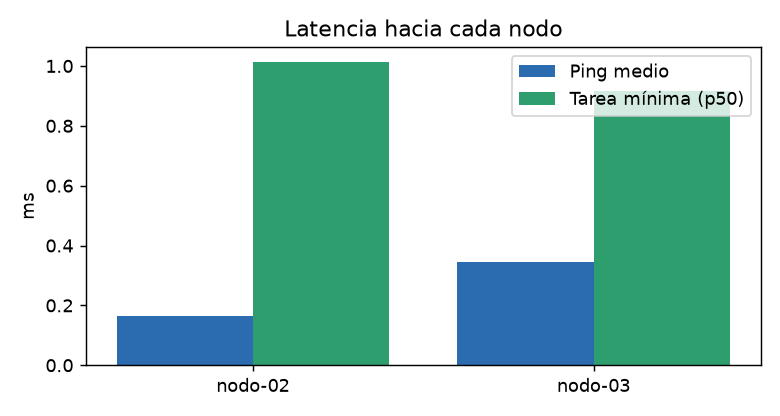
\includegraphics[width=0.7\textwidth]{figuras/latencia.png}
\caption{Latencia hacia cada nodo.}
\label{fig:latencia}
\end{figure}

\subsubsection{Tiempo de descubrimiento}

Se arranca un nodo nuevo, sin conocer a nadie, y se mide el tiempo hasta que descubre a todos los demás.

\begin{table}[htbp]
\centering
\small
\resizebox{\ifdim\width>\linewidth\linewidth\else\width\fi}{!}{%
\begin{tabular}{|c|c|c|c|}
\hline
\textbf{Intento} & \textbf{Segundos} & \textbf{Vecinos encontrados} & \textbf{Completo} \\ \hline
1 & 30.034 & 2 & no \\ \hline
2 & 30.038 & 2 & no \\ \hline
3 & 30.043 & 2 & no \\ \hline
4 & 0.203 & 3 & sí \\ \hline
5 & 0.102 & 3 & sí \\ \hline
6 & 0.101 & 3 & sí \\ \hline
7 & 0.102 & 3 & sí \\ \hline
8 & 0.101 & 3 & sí \\ \hline
\end{tabular}}
\caption{Tiempo de descubrimiento de un nodo nuevo.}
\label{tab:descubrimiento}
\end{table}

Descubrimiento completo en 5/8 intentos. En los 5 intentos completos tardó \textbf{0.12 s} de media (mín 0.10 s, máx 0.20 s). En los 3 restantes se agotó el límite de 30 s sin encontrar a todos los vecinos: el \emph{broadcast} UDP no tiene garantía de entrega y en una red Wi-Fi puede perderse; por eso el sistema también admite vecinos semilla por IP (\texttt{--peers}).

\subsubsection{Escalabilidad}

\paragraph{Más nodos, misma carga.} Se ejecuta el mismo lote de 24 tareas restringiendo el número de nodos disponibles.

\begin{table}[htbp]
\centering
\small
\resizebox{\ifdim\width>\linewidth\linewidth\else\width\fi}{!}{%
\begin{tabular}{|c|c|c|c|c|}
\hline
\textbf{Nodos} & \textbf{Tiempo total (s)} & \textbf{$\pm$ $\sigma$} & \textbf{Tareas/s} & \textbf{Aceleración} \\ \hline
1 & 2.621 & 0.26 & 9.26 & 1.0$\times$ \\ \hline
2 & 1.767 & 0.374 & 14.33 & 1.48$\times$ \\ \hline
3 & 1.69 & 0.137 & 14.29 & 1.55$\times$ \\ \hline
\end{tabular}}
\caption{Escalabilidad al aumentar el número de nodos.}
\label{tab:escal-nodos}
\end{table}

\begin{figure}[htbp]
\centering
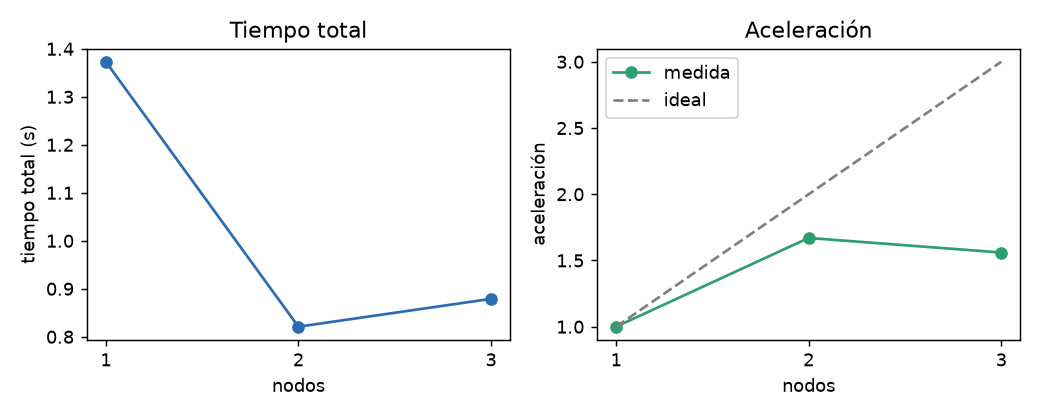
\includegraphics[width=0.9\textwidth]{figuras/escalabilidad_nodos.png}
\caption{Tiempo total y aceleración según el número de nodos.}
\label{fig:escal-nodos}
\end{figure}

Con 3 nodos la aceleración fue \textbf{1.55$\times$} (ideal: 3$\times$). La diferencia con el ideal se debe a la sobrecarga de coordinación (mensajes, ACK), a que las tareas se reparten en bloques discretos y a las diferencias de capacidad entre equipos.

\paragraph{Incremento progresivo de la carga.}

\begin{table}[htbp]
\centering
\small
\resizebox{\ifdim\width>\linewidth\linewidth\else\width\fi}{!}{%
\begin{tabular}{|c|c|c|c|c|c|c|}
\hline
\textbf{Tareas} & \textbf{Tiempo total (s)} & \textbf{Tareas/s} & \textbf{Latencia media (s)} & \textbf{p95 (s)} & \textbf{Tráfico enviado (KB/s)} & \textbf{CPU usada media (\%)} \\ \hline
4 & 0.222 & 17.99 & 0.197 & 0.221 & 6.79 & nodo-01: 24.5, nodo-03: 77.0, nodo-02: 20.2 \\ \hline
8 & 0.454 & 17.61 & 0.286 & 0.453 & 3.92 & nodo-01: 15.7, nodo-03: 77.0, nodo-02: 17.4 \\ \hline
16 & 1.291 & 12.4 & 0.487 & 0.898 & 2.71 & nodo-01: 21.1, nodo-03: 41.8, nodo-02: 17.4 \\ \hline
32 & 2.328 & 13.75 & 1.142 & 2.233 & 4.87 & nodo-01: 14.0, nodo-03: 52.6, nodo-02: 22.4 \\ \hline
64 & 4.417 & 14.49 & 1.455 & 3.801 & 3.57 & nodo-01: 17.3, nodo-03: 28.1, nodo-02: 23.4 \\ \hline
\end{tabular}}
\caption{Respuesta del sistema al aumentar la carga.}
\label{tab:escal-carga}
\end{table}

\begin{figure}[htbp]
\centering
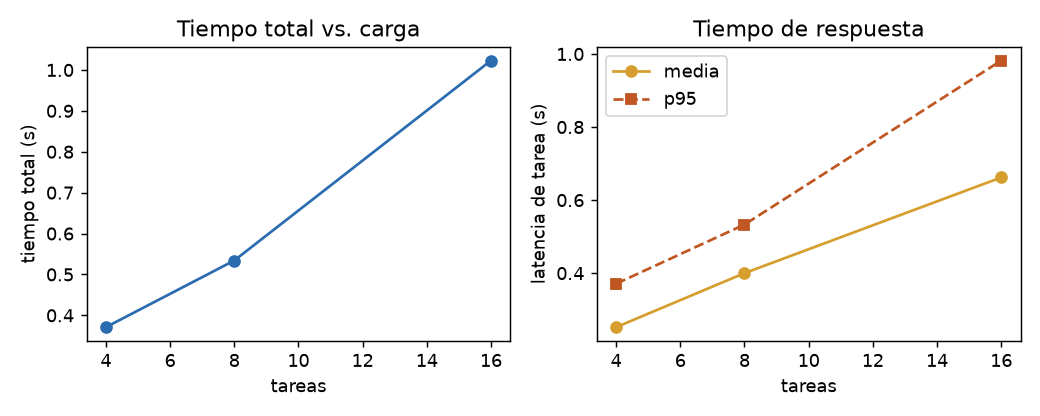
\includegraphics[width=0.9\textwidth]{figuras/carga_progresiva.png}
\caption{Tiempo total y tiempo de respuesta según la carga.}
\label{fig:escal-carga}
\end{figure}

Al multiplicar la carga por 16 (de 4 a 64 tareas) el tiempo total se multiplicó por 19.9 y el rendimiento pasó de 17.99 a 14.49 tareas/s. El tráfico de control fue de 3.57 KB/s con la mayor carga.

\subsubsection{Comparación de estrategias de asignación}

Mismo lote de 36 tareas de tamaño heterogéneo (0.5$\times$, 1$\times$ y 2$\times$) con cada estrategia. \emph{Desbalance} es el coeficiente de variación del número de tareas por nodo (0 = reparto perfecto).

\begin{table}[htbp]
\centering
\small
\resizebox{\ifdim\width>\linewidth\linewidth\else\width\fi}{!}{%
\begin{tabular}{|c|c|c|c|c|c|c|}
\hline
\textbf{Estrategia} & \textbf{Tiempo total (s)} & \textbf{$\pm$ $\sigma$} & \textbf{Latencia media (s)} & \textbf{p95 (s)} & \textbf{Desbalance} & \textbf{Tareas por nodo} \\ \hline
$F(i,j)$ del diseño & 5.029 & 2.334 & 2.621 & 4.929 & 1.414 & nodo-01: 0.0, nodo-02: 24.0, nodo-03: 12.0 \\ \hline
$F(i,j)$ + carga & 3.02 & 0.79 & 1.328 & 2.733 & 0.972 & nodo-01: 9.7, nodo-02: 20.7, nodo-03: 5.7 \\ \hline
Menos cargado & 2.948 & 0.408 & 0.944 & 2.603 & 0.0 & nodo-01: 12.0, nodo-02: 12.0, nodo-03: 12.0 \\ \hline
Menor latencia & 3.365 & 0.087 & 1.701 & 3.275 & 1.414 & nodo-01: 36.0, nodo-02: 0.0, nodo-03: 0.0 \\ \hline
Round-robin & 2.983 & 0.126 & 0.99 & 2.812 & 0.0 & nodo-01: 12.0, nodo-02: 12.0, nodo-03: 12.0 \\ \hline
Aleatoria & 3.078 & 0.34 & 1.011 & 2.855 & 0.203 & nodo-01: 9.7, nodo-02: 12.3, nodo-03: 14.0 \\ \hline
\end{tabular}}
\caption{Comparación de las seis estrategias de asignación.}
\label{tab:estrategias}
\end{table}

\begin{figure}[htbp]
\centering
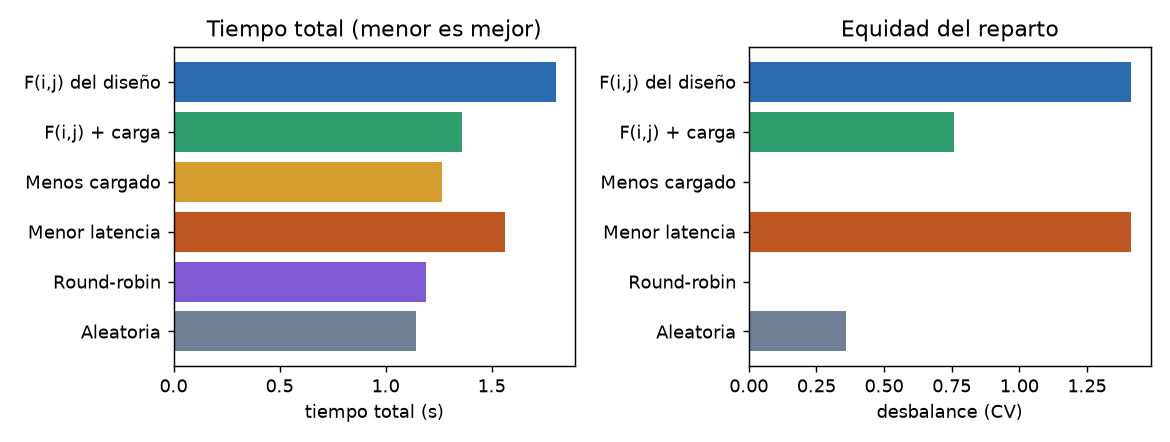
\includegraphics[width=0.9\textwidth]{figuras/estrategias.png}
\caption{Tiempo total y equidad del reparto por estrategia.}
\label{fig:estrategias}
\end{figure}

La estrategia con menor tiempo total fue \textbf{Menos cargado} (2.948 s) y la de mayor tiempo \textbf{$F(i,j)$ del diseño} (5.029 s). La función $F(i,j)$ del diseño original tardó 5.029 s con un desbalance de 1.414. Esa función no considera la carga actual y la normalización min-max convierte diferencias mínimas de CPU y memoria entre nodos desocupados en diferencias de 0 a 1, por lo que puede concentrar tareas en pocos nodos. La variante \texttt{weighted\_load} (término de carga y normalización robusta) redujo el tiempo total en 40\,\% y el desbalance de 1.414 a 0.972, conservando el criterio multicriterio.

\subsubsection{Tolerancia a fallos}

Un nodo cae 2 s después de empezar un lote de tareas (deja de enviar y recibir durante 25 s).

\begin{table}[htbp]
\centering
\small
\resizebox{\ifdim\width>\linewidth\linewidth\else\width\fi}{!}{%
\begin{tabular}{|c|c|c|c|c|c|c|c|c|}
\hline
\textbf{Intento} & \textbf{Nodo caído} & \textbf{Tareas} & \textbf{Completadas} & \textbf{\% completado} & \textbf{Reasignadas} & \textbf{Detección (s)} & \textbf{Recuperación (s)} & \textbf{Tiempo total (s)} \\ \hline
1 & nodo-02 & 20 & 20 & 100.0 & 10 & 4.25 & 4.16 & 10.41 \\ \hline
2 & nodo-03 & 20 & 20 & 100.0 & 4 & 5.38 & 1.22 & 8.61 \\ \hline
3 & nodo-02 & 20 & 20 & 100.0 & 15 & 4.31 & 6.06 & 12.38 \\ \hline
4 & nodo-03 & 20 & 20 & 100.0 & 4 & 4.98 & 1.18 & 8.17 \\ \hline
\end{tabular}}
\caption{Caída de un nodo durante la ejecución de un lote.}
\label{tab:fallos}
\end{table}

\begin{itemize}
\item Detección de la caída: media \textbf{4.73 s} (requisito: $\leq$ 5 s de silencio; la detección corre cada 0.5 s).
\item Tareas completadas pese a la caída: \textbf{100\,\%} (sin intervención manual).
\item La \emph{recuperación} es el tiempo desde la primera reasignación hasta que la tarea reasignada termina (incluye volver a ejecutarla).
\end{itemize}

\begin{figure}[htbp]
\centering
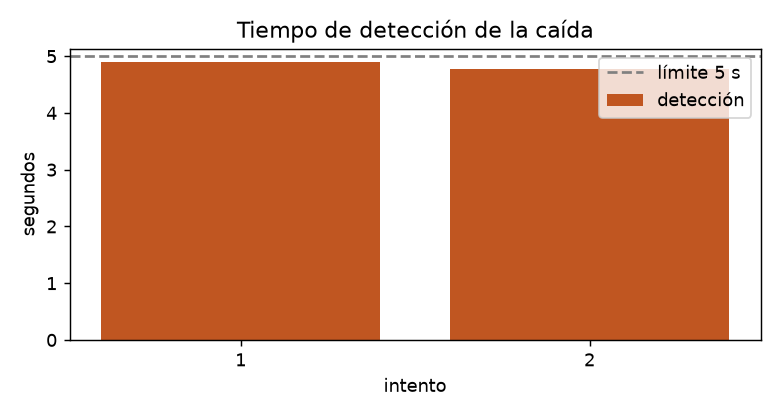
\includegraphics[width=0.7\textwidth]{figuras/tolerancia_fallos.png}
\caption{Tiempo de detección de la caída en cada intento.}
\label{fig:fallos}
\end{figure}

\subsubsection{Disponibilidad del servicio}

Cada 0.5 s se envía una tarea de sondeo mientras nodo-02 falla entre $t = 15$ s y $t = 35$ s.

\begin{table}[htbp]
\centering
\small
\resizebox{\ifdim\width>\linewidth\linewidth\else\width\fi}{!}{%
\begin{tabular}{|c|c|}
\hline
\textbf{Métrica} & \textbf{Valor} \\ \hline
Sondas enviadas & 140 \\ \hline
Completadas & 100.0 \% \\ \hline
Completadas en $\leq$ 3 s & 97.86 \% \\ \hline
\end{tabular}}
\caption{Disponibilidad del servicio durante la falla de un nodo.}
\label{tab:disponibilidad}
\end{table}

\begin{figure}[htbp]
\centering
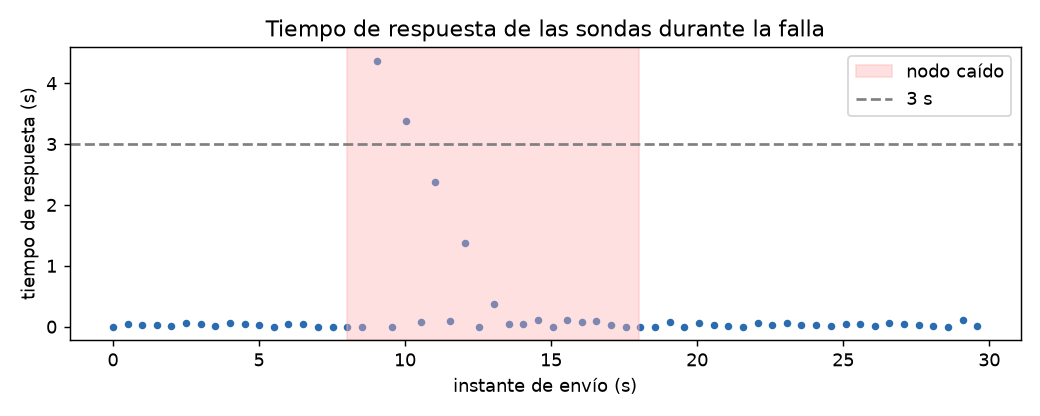
\includegraphics[width=0.9\textwidth]{figuras/disponibilidad.png}
\caption{Tiempo de respuesta de las sondas durante la falla.}
\label{fig:disponibilidad}
\end{figure}

Las sondas enviadas al nodo caído no reciben \texttt{TASK\_ACK}; tras el \emph{timeout} se reasignan a otro nodo y se completan, por eso la disponibilidad es alta pero algunas respuestas tardan alrededor del \emph{timeout} de 5 s.

\subsubsection{Consumo de recursos del nodo coordinador}

\begin{table}[htbp]
\centering
\small
\resizebox{\ifdim\width>\linewidth\linewidth\else\width\fi}{!}{%
\begin{tabular}{|c|c|}
\hline
\textbf{Métrica} & \textbf{Valor} \\ \hline
Mensajes enviados / recibidos & 2124 / 3469 \\ \hline
Tráfico enviado / recibido & 546 KB / 838 KB \\ \hline
Duración & 468 s \\ \hline
Tráfico medio enviado & 1.17 KB/s \\ \hline
Tareas enviadas / completadas / reasignadas / fallidas & 1308 / 1308 / 39 / 0 \\ \hline
\end{tabular}}
\caption{Consumo del nodo que coordinó los experimentos.}
\label{tab:recursos}
\end{table}

\subsubsection{Síntesis de los resultados}

\begin{itemize}
\item \textbf{Descubrimiento:} los nodos se encuentran solos en 0.12 s de media en 5/8 intentos, sin configuración manual.
\item \textbf{Escalabilidad:} con 3 nodos la aceleración fue 1.55$\times$ respecto a un solo nodo.
\item \textbf{Estrategias:} la de menor tiempo total fue Menos cargado.
\item \textbf{Fallos:} la caída se detectó en 4.73 s de media y se completó el 100\,\% de las tareas.
\item \textbf{Disponibilidad:} se completó el 100.0\,\% de las sondas durante la falla de un nodo.
\end{itemize}


\subsection{Pruebas}

El proyecto incluye 66 pruebas automáticas (\texttt{python -m pytest tests}): 42 de las fases anteriores
(planificador, mensajes, reloj de Lamport, tabla de vecinos, detector de fallos y escenarios de
integración con tres nodos reales) y 24 de la Fase 3, que verifican:

\begin{itemize}
\item las seis estrategias y su respeto por los requisitos de la tarea;
\item la normalización robusta (sin amplificar diferencias mínimas) y el ejemplo numérico del diseño;
\item que la suma de los estadísticos de los fragmentos equivale a la regresión sobre todos los datos;
\item la API (\texttt{map} conserva el orden, el requisito de nodos, el cambio de estrategia, \texttt{on\_event});
\item que una alerta llega al registro de todos los nodos;
\item que un nodo caído pasa a \texttt{OFFLINE}, se recupera y que sus tareas se reasignan;
\item que las ranuras limitan la ejecución simultánea y la detección de la subred.
\end{itemize}

\subsection{Qué se puede demostrar en la sustentación}

\begin{itemize}
\item Tres computadores físicos descubriéndose automáticamente en la misma red.
\item El panel web mostrando los tres nodos, sus recursos, la latencia y las tareas en vivo.
\item Las tres aplicaciones: alertas de monitoreo, procesamiento \emph{map-reduce} y regresión
lineal distribuida.
\item La caída de un nodo durante una tarea: alerta crítica, reasignación automática y resultado
correcto.
\item El cambio de estrategia de asignación en caliente y su efecto en el reparto.
\item Las métricas y gráficas de los experimentos.
\end{itemize}

\subsection{Limitaciones}

\begin{itemize}
\item El ancho de banda de cada nodo es un valor declarado, no medido.
\item UDP no garantiza la entrega ni hay retransmisión: la pérdida de un mensaje se maneja con el
\emph{timeout} de la confirmación y la reasignación de la tarea.
\item El nodo que envía una tarea la coordina; si ese nodo cae, pierde el estado de sus tareas, porque
no hay persistencia.
\item La sincronización es un orden lógico de eventos (Lamport); no hay exclusión mutua distribuida.
\item Los \emph{endpoints} de administración no tienen autenticación (uso de laboratorio).
\item Las tareas deben ser lo bastante grandes para amortizar el costo de la comunicación.
\end{itemize}

\subsection{Conclusión de la fase}

Con esta fase se completa ComplexNet API: una red de tres computadores físicos que se descubren solos,
reparten el trabajo con reglas locales, ejecutan aplicaciones de monitoreo, procesamiento y
aprendizaje automático distribuido, detectan fallos y se recuperan sin intervención humana ni
coordinador central. La API permite a otros desarrolladores crear nuevas aplicaciones con pocas líneas,
y la evaluación experimental respalda el comportamiento del sistema en latencia, escalabilidad,
disponibilidad y tolerancia a fallos. Del análisis de las estrategias de asignación resultó una mejora
al modelo original (normalización robusta y término de carga) que evita concentrar las tareas en un
solo nodo.

% Requiere solo el paquete graphicx (ya usado en las secciones anteriores).
% Las tablas y figuras de resultados se generan con
%         python experiments/report.py
% en el archivo fase3_resultados.tex (se incluye al final de esta sección).
% =============================================================================

\section{Descripción del Proyecto -- Fase 3}

\subsection{Objetivo de la fase}

En la Fase 2 se construyó el núcleo de ComplexNet API y se validó con tres nodos en contenedores
Docker dentro de un mismo computador. La Fase 3 convierte ese núcleo en una plataforma utilizable:
se ejecuta sobre \textbf{tres computadores físicos} conectados por una red local, ofrece una
\textbf{API documentada para desarrolladores}, incluye \textbf{tres aplicaciones descentralizadas}
construidas sobre ella, un \textbf{panel de monitoreo} del clúster y una \textbf{evaluación
experimental} de latencia, escalabilidad, disponibilidad, tolerancia a fallos y estrategias de
asignación de tareas.

\subsection{Qué se agregó respecto a la Fase 2}

El núcleo (mensajes JSON sobre UDP, descubrimiento por \emph{beacons}, detección de fallos por
silencio, reasignación de tareas y reloj lógico de Lamport) se mantiene. Lo nuevo es lo siguiente:

\begin{table}[htbp]
\centering
\small
\begin{tabular}{|p{0.2\textwidth}|p{0.33\textwidth}|p{0.33\textwidth}|}
\hline
\textbf{Aspecto} & \textbf{Fase 2} & \textbf{Fase 3} \\ \hline
Despliegue & Tres contenedores Docker en un computador, red virtual & Tres computadores físicos en una red local real \\ \hline
Descubrimiento & \emph{Broadcast} a una subred fija de Docker & Detección automática de la subred y vecinos semilla por IP \\ \hline
Uso del sistema & Script de demostración & API para desarrolladores y manual \\ \hline
Aplicaciones & Una tarea de regresión lineal de ejemplo & Tres aplicaciones descentralizadas \\ \hline
Monitoreo & Terminal y un archivo JSON por nodo & Panel web en vivo con alertas \\ \hline
Planificación & Una función de aptitud $F(i,j)$ & Seis estrategias intercambiables en caliente \\ \hline
Capacidad del nodo & Sin límite de tareas simultáneas & Ranuras de ejecución (\emph{slots}) y cola \\ \hline
Validación & Pruebas funcionales (42) & Pruebas (66) y experimentos con informe \\ \hline
\end{tabular}
\caption{Cambios de la Fase 3 respecto a la Fase 2.}
\label{tab:fase2-fase3}
\end{table}

\subsection{Despliegue en tres computadores}

\paragraph{¿Cómo se conectan los computadores?}
Los tres equipos se conectan a la \textbf{misma red local} (mismo Wi-Fi o router; también sirve el
punto de acceso de un celular). No se usa ningún servidor central ni se necesita internet: cada
nodo envía los mensajes directamente a los demás mediante \textbf{UDP sobre IP}, por el puerto
\texttt{9999}. El panel web usa el puerto \texttt{8000} (TCP) y es solo para observar y administrar.

\begin{table}[htbp]
\centering
\small
\begin{tabular}{|c|c|p{0.5\textwidth}|}
\hline
\textbf{Equipo} & \textbf{Nodo} & \textbf{Qué ejecuta} \\ \hline
Computador 1 & \texttt{nodo-01} & Un nodo, las aplicaciones y los experimentos \\ \hline
Computador 2 & \texttt{nodo-02} & Solo el nodo \\ \hline
Computador 3 & \texttt{nodo-03} & Solo el nodo \\ \hline
\end{tabular}
\caption{Distribución de nodos en los computadores.}
\label{tab:tres-pcs}
\end{table}

\paragraph{Descubrimiento en la red real.}
\begin{enumerate}
\item Cada nodo emite cada 2 s un mensaje \texttt{RESOURCE\_BEACON} por \emph{broadcast} UDP, es decir,
a la dirección que reciben todos los equipos de la subred. El nodo calcula esa dirección a partir de
su propia IP y máscara de red (opción \texttt{--broadcast auto}).
\item El \emph{beacon} informa el identificador del nodo, su IP, su CPU libre, su memoria libre, su ancho
de banda y cuántas tareas tiene en curso.
\item Al recibir el \emph{beacon} de un nodo desconocido, el receptor lo registra en su \texttt{PeerTable}
y le responde con un \emph{beacon} directo. Así, basta con que uno de los dos oiga al otro para que
ambos se descubran.
\item Si la red bloquea el \emph{broadcast} (algunas redes institucionales lo filtran), cada nodo puede
iniciarse con las IP de sus vecinos (\texttt{--peers}) y los mensajes viajan de forma directa. Otra
alternativa es conectar los tres equipos al punto de acceso de un celular.
\end{enumerate}

\paragraph{Mensajes del protocolo.}
Todos los mensajes son JSON con un encabezado (identificador único, emisor, tipo, marca de tiempo y
reloj de Lamport) y una carga útil. El tamaño máximo es de 60 KB, de modo que cada mensaje cabe en un
datagrama UDP.

\begin{table}[htbp]
\centering
\small
\begin{tabular}{|l|p{0.55\textwidth}|}
\hline
\textbf{Mensaje} & \textbf{Función} \\ \hline
\texttt{RESOURCE\_BEACON} & Presencia y recursos del nodo (cada 2 s) \\ \hline
\texttt{PING} / \texttt{PONG} & Medición de la latencia (RTT) entre dos nodos \\ \hline
\texttt{TASK\_SUBMIT} & Envío de una tarea al nodo elegido \\ \hline
\texttt{TASK\_ACK} & Confirmación de recepción de la tarea \\ \hline
\texttt{TASK\_RESULT} & Resultado de la tarea o error \\ \hline
\texttt{ALERT} & Alerta difundida a todos los nodos (Fase 3) \\ \hline
\end{tabular}
\caption{Mensajes intercambiados entre los nodos.}
\label{tab:mensajes}
\end{table}

\paragraph{Puesta en marcha.}
Cada computador ejecuta un único comando, que crea el entorno de Python, instala las dependencias,
abre el puerto en el cortafuegos y arranca el nodo:

\begin{verbatim}
.\scripts\start_node.ps1 -Id nodo-02
\end{verbatim}

\subsection{API para desarrolladores}

La clase \texttt{Node} es la puerta de entrada: oculta el descubrimiento, la planificación, la
comunicación y la recuperación ante fallos. Una aplicación necesita pocas líneas:

\begin{verbatim}
from complexnet import Node, Task

with Node("nodo-01", broadcast_address="auto") as node:
    node.wait_for_peers(2)
    tarea = Task("regresion_lineal", {"n_samples": 10000},
                 requirements={"cpu": 1, "memory": 256})
    resultado = node.submit(tarea)      # el planificador elige el nodo
\end{verbatim}

\begin{table}[htbp]
\centering
\small
\begin{tabular}{|p{0.3\textwidth}|p{0.6\textwidth}|}
\hline
\textbf{Método} & \textbf{Descripción} \\ \hline
\texttt{connect()}, \texttt{disconnect()} & Une el nodo a la red o lo detiene (también como \texttt{with}) \\ \hline
\texttt{wait\_for\_peers(n)} & Espera hasta tener $n$ vecinos activos \\ \hline
\texttt{submit(tarea)} & Envía una tarea y devuelve su resultado (o la tarea, sin esperar) \\ \hline
\texttt{map(nombre, lista)} & Una tarea por elemento; devuelve los resultados en orden \\ \hline
\texttt{map\_tasks(...)} & Igual que \texttt{map}, pero devuelve las tareas con sus tiempos y el nodo ejecutor \\ \hline
\texttt{broadcast(tipo, datos)} & Envía un mensaje a todos los vecinos activos \\ \hline
\texttt{raise\_alert(nivel, texto)} & Registra una alerta y la difunde a toda la red \\ \hline
\texttt{on\_event(funcion)} & Ejecuta una función por cada evento del nodo (fallos, tareas, descubrimiento) \\ \hline
\texttt{set\_strategy(nombre)} & Cambia la estrategia de asignación en caliente \\ \hline
\texttt{simulate\_failure(s)} & Simula una caída del nodo durante $s$ segundos (pruebas) \\ \hline
\texttt{status()} & Estado completo: recursos, vecinos, tareas, alertas y métricas \\ \hline
\end{tabular}
\caption{Métodos principales de la API.}
\label{tab:api}
\end{table}

Una \texttt{Task} lleva un nombre, sus parámetros y requisitos (CPU libre mínima, memoria mínima y,
opcionalmente, una lista de nodos permitidos). Los tipos de tarea disponibles son los siguientes:

\begin{table}[htbp]
\centering
\small
\begin{tabular}{|l|p{0.55\textwidth}|}
\hline
\textbf{Tarea} & \textbf{Descripción} \\ \hline
\texttt{regresion\_lineal} & Regresión lineal completa en un nodo (Fase 2) \\ \hline
\texttt{normal\_equations} & Estadísticos de un fragmento de datos para la regresión distribuida \\ \hline
\texttt{evaluate\_model} & Evaluación de un modelo sobre un fragmento de datos \\ \hline
\texttt{monte\_carlo\_pi} & Estimación de $\pi$ por el método de Monte Carlo \\ \hline
\texttt{word\_count} & Conteo de palabras de un fragmento de texto \\ \hline
\end{tabular}
\caption{Tipos de tarea incluidos.}
\label{tab:tareas}
\end{table}

Agregar una tarea nueva consiste en escribir una función de Python que reciba un diccionario y
devuelva otro, y registrarla en el módulo de ejecutores. La referencia completa está en el manual del
desarrollador (\texttt{docs/api/MANUAL\_DESARROLLADOR.md}).

\subsection{Aplicaciones descentralizadas}

Las tres aplicaciones usan únicamente la API anterior; ninguna depende de un servidor central.

\subsubsection{Aplicación 1: monitoreo distribuido con alertas}

Vigila el clúster con la información que ya circula en los \emph{beacons} y genera alertas que se
\textbf{difunden a todos los nodos}, de modo que cada nodo conserva su propio registro de alertas.

\begin{itemize}
\item \textbf{Crítica:} un nodo pasa a \texttt{OFFLINE}.
\item \textbf{Informativa:} un nodo vuelve a estar \texttt{ONLINE}.
\item \textbf{Advertencia:} CPU libre menor a un umbral, memoria libre menor a un umbral o latencia
mayor a un umbral (configurables).
\end{itemize}

Además guarda una serie de tiempo con la CPU, la memoria y la latencia de cada nodo, y las alertas
aparecen en el panel web.

\subsubsection{Aplicación 2: procesamiento distribuido}

Realiza dos trabajos de tipo \emph{map-reduce} repartidos por la red:

\begin{enumerate}
\item \textbf{Análisis de archivos:} los archivos de texto de una carpeta se parten en fragmentos; cada
nodo cuenta las palabras de su fragmento (\emph{map}) y el nodo coordinador combina los conteos
(\emph{reduce}).
\item \textbf{Cálculo colaborativo:} estimación de $\pi$ por Monte Carlo. Cada nodo lanza puntos al azar
en el cuadrado unidad y cuenta los que caen dentro del círculo; con el total se obtiene
$\pi \approx 4 \cdot \mathrm{dentro} / \mathrm{total}$.
\end{enumerate}

Si un nodo cae durante el trabajo, sus fragmentos se reasignan y el resultado no cambia.

\subsubsection{Aplicación 3: inteligencia artificial distribuida}

Entrena una \textbf{regresión lineal múltiple} repartiendo los datos entre los nodos. La idea es que
la solución de mínimos cuadrados se puede calcular a partir de sumas parciales. Si el conjunto de
datos se divide en fragmentos $(X_k, y_k)$, cada nodo calcula $X_k^{\top}X_k$ y $X_k^{\top}y_k$ de su
fragmento y el coordinador los suma y resuelve:

\begin{equation}
\hat{w} = \Bigl(\sum_k X_k^{\top}X_k\Bigr)^{-1} \sum_k X_k^{\top}y_k
\end{equation}

El resultado es exactamente el de entrenar con todos los datos en un solo equipo. Cada fragmento se
genera dentro del nodo que lo procesa a partir de una semilla, por lo que por la red solo viajan
parámetros pequeños y estadísticos. El modelo se evalúa después en fragmentos nuevos, también
repartidos, calculando el coeficiente de determinación
$R^2 = 1 - \mathrm{SSE}/\mathrm{SST}$. Si un nodo falla durante el entrenamiento, su fragmento se
reasigna a otro y los pesos finales son los mismos.

\begin{table}[htbp]
\centering
\small
\begin{tabular}{|p{0.28\textwidth}|p{0.62\textwidth}|}
\hline
\textbf{Requisito del taller} & \textbf{Cómo se cumple} \\ \hline
Distribución de datos & Fragmentos generados en cada nodo a partir de una semilla \\ \hline
Asignación de recursos & El planificador reparte cada fragmento según CPU, memoria, ancho de banda, latencia, reputación y carga \\ \hline
Información intercambiada & Estadísticos $X_k^{\top}X_k$, $X_k^{\top}y_k$ y sumas de cuadrados, no los datos \\ \hline
Métricas & Error de los pesos, $R^2$, MSE, tiempos y fragmentos por nodo \\ \hline
Tolerancia a fallos & Reasignación automática del fragmento del nodo caído \\ \hline
\end{tabular}
\caption{Aplicación de inteligencia artificial: cumplimiento de los requisitos.}
\label{tab:ia}
\end{table}

\subsection{Estrategias de asignación de tareas}

El planificador de la Fase 2 implementa la función de aptitud del diseño (sección 9):

\begin{equation}
F(i,j) = 0.40\,C' + 0.40\,M' + 0.10\,B' + 0.05\,R - 0.05\,(1 - L')
\end{equation}

donde $C'$, $M'$, $B'$ y $L'$ son la CPU libre, la memoria libre, el ancho de banda y la latencia
(esta última con normalización inversa) normalizados entre los candidatos, y $R$ es la reputación del
nodo. Al probarla en los experimentos se observó un problema: la normalización min-max convierte
diferencias mínimas entre nodos casi idénticos (por ejemplo, 1\,\% de CPU) en diferencias de 0 a 1, y
la función no conoce cuántas tareas tiene ya cada nodo, así que podía enviar todas las tareas al mismo
nodo.

Para resolverlo se agregó la variante \texttt{weighted\_load}, que usa por defecto:

\begin{itemize}
\item \textbf{Normalización robusta:} $x' = (x - \min x) / \max(\max x - \min x,\ \delta)$, donde
$\delta$ es un rango mínimo significativo ($\delta_C = 20$ puntos de CPU libre, $\delta_M = \delta_B = 20\,\%$
del mayor valor y $\delta_L = 5$ ms). Las diferencias de ruido ya no se amplifican.
\item \textbf{Término de carga:} se resta $0.30\,Q'$, donde $Q'$ es el número de tareas en curso del
nodo (incluidas las que el propio coordinador le acaba de enviar) normalizado entre los candidatos; los
pesos de CPU y memoria bajan a 0.25 para que la suma siga siendo 1.
\end{itemize}

\begin{equation}
F_{L}(i,j) = 0.25\,C' + 0.25\,M' + 0.10\,B' + 0.05\,R - 0.05\,(1 - L') - 0.30\,Q'
\end{equation}

Además se implementaron cuatro estrategias de referencia para compararlas:

\begin{table}[htbp]
\centering
\small
\begin{tabular}{|l|p{0.6\textwidth}|}
\hline
\textbf{Estrategia} & \textbf{Criterio} \\ \hline
\texttt{weighted} & $F(i,j)$ del diseño \\ \hline
\texttt{weighted\_load} & $F_L(i,j)$: robusta y con carga (por defecto) \\ \hline
\texttt{least\_loaded} & El nodo con menos tareas en curso \\ \hline
\texttt{lowest\_latency} & El nodo con menor latencia medida \\ \hline
\texttt{round\_robin} & Reparto cíclico entre los candidatos aptos \\ \hline
\texttt{random} & Un candidato apto al azar \\ \hline
\end{tabular}
\caption{Estrategias de asignación implementadas.}
\label{tab:estrategias-lista}
\end{table}

En todas, el conjunto de candidatos se filtra primero con los requisitos de la tarea
($C_i \geq C_{\mathrm{req}}$ y $M_i \geq M_{\mathrm{req}}$) y solo se consideran los nodos activos.

\paragraph{Capacidad de los nodos.}
Cada nodo ejecuta como máximo \texttt{slots} tareas a la vez (2 por defecto); las demás esperan en cola.
Esto modela un computador con CPU limitada y hace que el reparto de carga sea relevante.

\subsection{Panel de monitoreo del clúster}

Cada nodo sirve una página web (\texttt{http://IP-DEL-NODO:8000}) que muestra, en tiempo real, los
nodos del clúster con su estado, CPU, memoria y latencia, la evolución de la latencia, las tareas y sus
resultados, las alertas y el registro de eventos. El mismo servicio expone una API HTTP: consulta del
estado (\texttt{GET /status}, \texttt{GET /events}), envío de tareas (\texttt{POST /tasks}) y
administración para los experimentos (\texttt{POST /admin/fail} para simular una caída remota y
\texttt{POST /admin/strategy} para cambiar la estrategia).

\subsection{Metodología experimental}

Los experimentos se ejecutan con \texttt{experiments/run\_experiments.py} desde el computador 1 y el
informe se genera con \texttt{experiments/report.py} a partir de los archivos CSV resultantes. La carga
de trabajo son tareas de Monte Carlo (intensivas en CPU), y cada medición se repite varias veces para
reportar la media y la desviación estándar. Se evalúan:

\begin{itemize}
\item \textbf{Latencia:} RTT de \texttt{PING}/\texttt{PONG} y tiempo de una tarea mínima.
\item \textbf{Tiempo de descubrimiento:} desde que arranca un nodo nuevo hasta conocer a los demás.
\item \textbf{Escalabilidad:} el mismo lote con 1, 2 y 3 nodos (aceleración) y cargas crecientes.
\item \textbf{Estrategias de asignación:} el mismo lote heterogéneo con las seis estrategias.
\item \textbf{Tolerancia a fallos:} un nodo cae a mitad de un lote y se mide la detección, la
recuperación y el porcentaje de tareas completadas.
\item \textbf{Disponibilidad:} se envía una tarea de sondeo cada 0.5 s mientras un nodo falla.
\end{itemize}

Las fallas se inyectan con el endpoint \texttt{/admin/fail} del nodo víctima, que deja de enviar y
recibir mensajes durante unos segundos, lo que equivale a una caída o a una desconexión de la red.

\subsection{Resultados experimentales}

Las tablas y gráficas de esta sección se generan automáticamente a partir de los datos medidos.

% ARCHIVO GENERADO por experiments/report.py -- no editar a mano.
% Corrida: 20261126-104206

\subsubsection{Entorno}

\begin{table}[htbp]
\centering
\small
\resizebox{\ifdim\width>\linewidth\linewidth\else\width\fi}{!}{%
\begin{tabular}{|c|c|}
\hline
\textbf{Dato} & \textbf{Valor} \\ \hline
Fecha & 2026-11-26 10:42:06 \\ \hline
Entorno & 3 computadores en red local \\ \hline
Nodos & nodo-01 (172.25.4.83), nodo-03 (172.25.5.66), nodo-02 (172.25.7.119) \\ \hline
Equipo que ejecutó los experimentos & MSI (Windows-11-10.0.26200-SP0) \\ \hline
CPU / RAM de ese equipo & 12 hilos / 15.7 GB \\ \hline
Python & 3.13.7 \\ \hline
Estrategia por defecto & weighted\_load \\ \hline
Tamaño de tarea (puntos Monte Carlo) & 12,000,000 \\ \hline
Modo & completo \\ \hline
\end{tabular}}
\caption{Entorno de la corrida experimental.}
\label{tab:entorno}
\end{table}

Los experimentos se ejecutaron en \textbf{tres computadores físicos} conectados a la misma red local, un nodo por computador.

\subsubsection{Latencia de comunicación}

\begin{table}[htbp]
\centering
\small
\resizebox{\ifdim\width>\linewidth\linewidth\else\width\fi}{!}{%
\begin{tabular}{|c|c|c|c|c|c|}
\hline
\textbf{Nodo} & \textbf{Ping medio (ms)} & \textbf{Ping mín (ms)} & \textbf{Ping máx (ms)} & \textbf{Tarea mínima p50 (ms)} & \textbf{Tarea mínima p95 (ms)} \\ \hline
nodo-02 & 61.116 & 30.221 & 136.877 & 7.733 & 26.384 \\ \hline
nodo-03 & 24.971 & 16.617 & 38.265 & 9.414 & 21.802 \\ \hline
\end{tabular}}
\caption{Latencia hacia cada nodo.}
\label{tab:latencia}
\end{table}

\emph{Ping} es el RTT de los mensajes \texttt{PING}/\texttt{PONG} que cada nodo mide a sus vecinos. \emph{Tarea mínima} es el tiempo completo de una tarea \texttt{echo} (asignación, envío, ejecución y respuesta).

\begin{figure}[htbp]
\centering
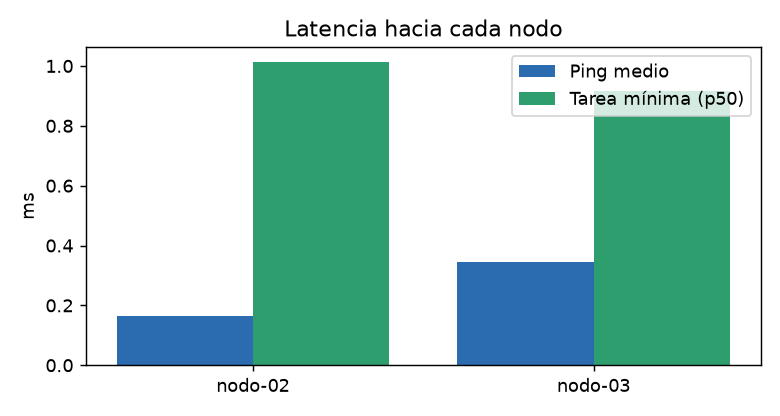
\includegraphics[width=0.7\textwidth]{figuras/latencia.png}
\caption{Latencia hacia cada nodo.}
\label{fig:latencia}
\end{figure}

\subsubsection{Tiempo de descubrimiento}

Se arranca un nodo nuevo, sin conocer a nadie, y se mide el tiempo hasta que descubre a todos los demás.

\begin{table}[htbp]
\centering
\small
\resizebox{\ifdim\width>\linewidth\linewidth\else\width\fi}{!}{%
\begin{tabular}{|c|c|c|c|}
\hline
\textbf{Intento} & \textbf{Segundos} & \textbf{Vecinos encontrados} & \textbf{Completo} \\ \hline
1 & 30.034 & 2 & no \\ \hline
2 & 30.038 & 2 & no \\ \hline
3 & 30.043 & 2 & no \\ \hline
4 & 0.203 & 3 & sí \\ \hline
5 & 0.102 & 3 & sí \\ \hline
6 & 0.101 & 3 & sí \\ \hline
7 & 0.102 & 3 & sí \\ \hline
8 & 0.101 & 3 & sí \\ \hline
\end{tabular}}
\caption{Tiempo de descubrimiento de un nodo nuevo.}
\label{tab:descubrimiento}
\end{table}

Descubrimiento completo en 5/8 intentos. En los 5 intentos completos tardó \textbf{0.12 s} de media (mín 0.10 s, máx 0.20 s). En los 3 restantes se agotó el límite de 30 s sin encontrar a todos los vecinos: el \emph{broadcast} UDP no tiene garantía de entrega y en una red Wi-Fi puede perderse; por eso el sistema también admite vecinos semilla por IP (\texttt{--peers}).

\subsubsection{Escalabilidad}

\paragraph{Más nodos, misma carga.} Se ejecuta el mismo lote de 24 tareas restringiendo el número de nodos disponibles.

\begin{table}[htbp]
\centering
\small
\resizebox{\ifdim\width>\linewidth\linewidth\else\width\fi}{!}{%
\begin{tabular}{|c|c|c|c|c|}
\hline
\textbf{Nodos} & \textbf{Tiempo total (s)} & \textbf{$\pm$ $\sigma$} & \textbf{Tareas/s} & \textbf{Aceleración} \\ \hline
1 & 2.621 & 0.26 & 9.26 & 1.0$\times$ \\ \hline
2 & 1.767 & 0.374 & 14.33 & 1.48$\times$ \\ \hline
3 & 1.69 & 0.137 & 14.29 & 1.55$\times$ \\ \hline
\end{tabular}}
\caption{Escalabilidad al aumentar el número de nodos.}
\label{tab:escal-nodos}
\end{table}

\begin{figure}[htbp]
\centering
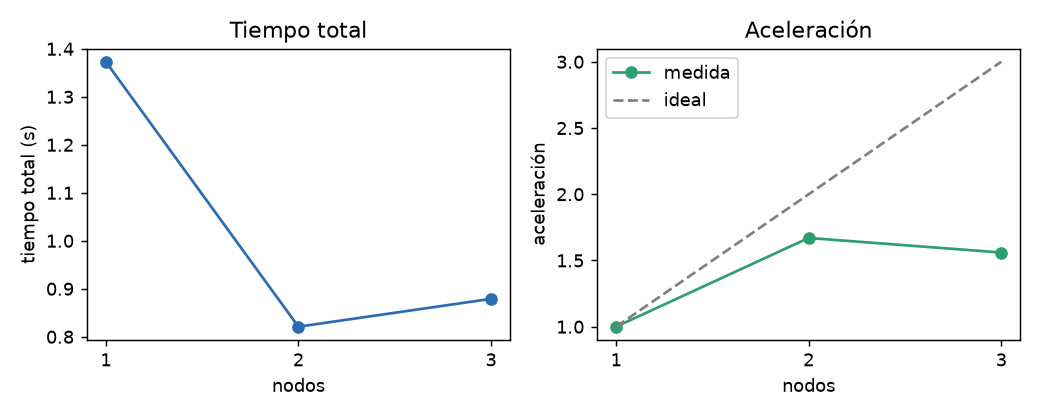
\includegraphics[width=0.9\textwidth]{figuras/escalabilidad_nodos.png}
\caption{Tiempo total y aceleración según el número de nodos.}
\label{fig:escal-nodos}
\end{figure}

Con 3 nodos la aceleración fue \textbf{1.55$\times$} (ideal: 3$\times$). La diferencia con el ideal se debe a la sobrecarga de coordinación (mensajes, ACK), a que las tareas se reparten en bloques discretos y a las diferencias de capacidad entre equipos.

\paragraph{Incremento progresivo de la carga.}

\begin{table}[htbp]
\centering
\small
\resizebox{\ifdim\width>\linewidth\linewidth\else\width\fi}{!}{%
\begin{tabular}{|c|c|c|c|c|c|c|}
\hline
\textbf{Tareas} & \textbf{Tiempo total (s)} & \textbf{Tareas/s} & \textbf{Latencia media (s)} & \textbf{p95 (s)} & \textbf{Tráfico enviado (KB/s)} & \textbf{CPU usada media (\%)} \\ \hline
4 & 0.222 & 17.99 & 0.197 & 0.221 & 6.79 & nodo-01: 24.5, nodo-03: 77.0, nodo-02: 20.2 \\ \hline
8 & 0.454 & 17.61 & 0.286 & 0.453 & 3.92 & nodo-01: 15.7, nodo-03: 77.0, nodo-02: 17.4 \\ \hline
16 & 1.291 & 12.4 & 0.487 & 0.898 & 2.71 & nodo-01: 21.1, nodo-03: 41.8, nodo-02: 17.4 \\ \hline
32 & 2.328 & 13.75 & 1.142 & 2.233 & 4.87 & nodo-01: 14.0, nodo-03: 52.6, nodo-02: 22.4 \\ \hline
64 & 4.417 & 14.49 & 1.455 & 3.801 & 3.57 & nodo-01: 17.3, nodo-03: 28.1, nodo-02: 23.4 \\ \hline
\end{tabular}}
\caption{Respuesta del sistema al aumentar la carga.}
\label{tab:escal-carga}
\end{table}

\begin{figure}[htbp]
\centering
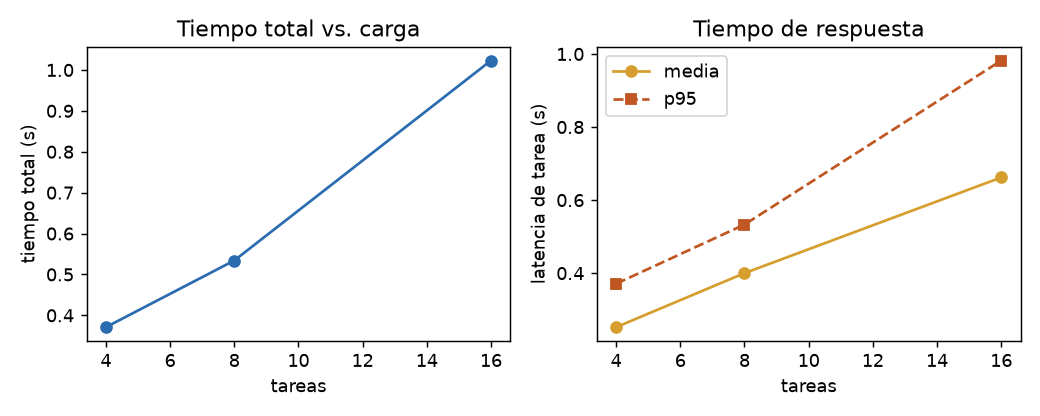
\includegraphics[width=0.9\textwidth]{figuras/carga_progresiva.png}
\caption{Tiempo total y tiempo de respuesta según la carga.}
\label{fig:escal-carga}
\end{figure}

Al multiplicar la carga por 16 (de 4 a 64 tareas) el tiempo total se multiplicó por 19.9 y el rendimiento pasó de 17.99 a 14.49 tareas/s. El tráfico de control fue de 3.57 KB/s con la mayor carga.

\subsubsection{Comparación de estrategias de asignación}

Mismo lote de 36 tareas de tamaño heterogéneo (0.5$\times$, 1$\times$ y 2$\times$) con cada estrategia. \emph{Desbalance} es el coeficiente de variación del número de tareas por nodo (0 = reparto perfecto).

\begin{table}[htbp]
\centering
\small
\resizebox{\ifdim\width>\linewidth\linewidth\else\width\fi}{!}{%
\begin{tabular}{|c|c|c|c|c|c|c|}
\hline
\textbf{Estrategia} & \textbf{Tiempo total (s)} & \textbf{$\pm$ $\sigma$} & \textbf{Latencia media (s)} & \textbf{p95 (s)} & \textbf{Desbalance} & \textbf{Tareas por nodo} \\ \hline
$F(i,j)$ del diseño & 5.029 & 2.334 & 2.621 & 4.929 & 1.414 & nodo-01: 0.0, nodo-02: 24.0, nodo-03: 12.0 \\ \hline
$F(i,j)$ + carga & 3.02 & 0.79 & 1.328 & 2.733 & 0.972 & nodo-01: 9.7, nodo-02: 20.7, nodo-03: 5.7 \\ \hline
Menos cargado & 2.948 & 0.408 & 0.944 & 2.603 & 0.0 & nodo-01: 12.0, nodo-02: 12.0, nodo-03: 12.0 \\ \hline
Menor latencia & 3.365 & 0.087 & 1.701 & 3.275 & 1.414 & nodo-01: 36.0, nodo-02: 0.0, nodo-03: 0.0 \\ \hline
Round-robin & 2.983 & 0.126 & 0.99 & 2.812 & 0.0 & nodo-01: 12.0, nodo-02: 12.0, nodo-03: 12.0 \\ \hline
Aleatoria & 3.078 & 0.34 & 1.011 & 2.855 & 0.203 & nodo-01: 9.7, nodo-02: 12.3, nodo-03: 14.0 \\ \hline
\end{tabular}}
\caption{Comparación de las seis estrategias de asignación.}
\label{tab:estrategias}
\end{table}

\begin{figure}[htbp]
\centering
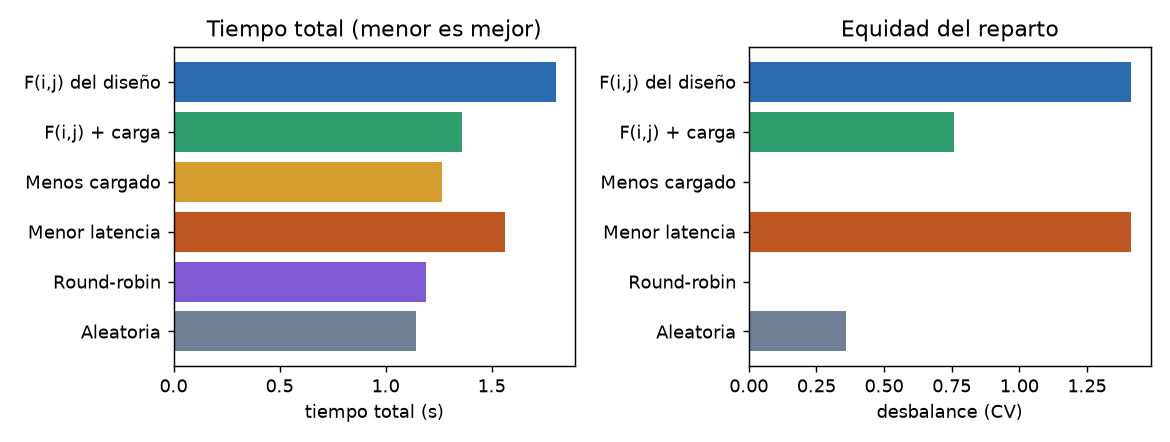
\includegraphics[width=0.9\textwidth]{figuras/estrategias.png}
\caption{Tiempo total y equidad del reparto por estrategia.}
\label{fig:estrategias}
\end{figure}

La estrategia con menor tiempo total fue \textbf{Menos cargado} (2.948 s) y la de mayor tiempo \textbf{$F(i,j)$ del diseño} (5.029 s). La función $F(i,j)$ del diseño original tardó 5.029 s con un desbalance de 1.414. Esa función no considera la carga actual y la normalización min-max convierte diferencias mínimas de CPU y memoria entre nodos desocupados en diferencias de 0 a 1, por lo que puede concentrar tareas en pocos nodos. La variante \texttt{weighted\_load} (término de carga y normalización robusta) redujo el tiempo total en 40\,\% y el desbalance de 1.414 a 0.972, conservando el criterio multicriterio.

\subsubsection{Tolerancia a fallos}

Un nodo cae 2 s después de empezar un lote de tareas (deja de enviar y recibir durante 25 s).

\begin{table}[htbp]
\centering
\small
\resizebox{\ifdim\width>\linewidth\linewidth\else\width\fi}{!}{%
\begin{tabular}{|c|c|c|c|c|c|c|c|c|}
\hline
\textbf{Intento} & \textbf{Nodo caído} & \textbf{Tareas} & \textbf{Completadas} & \textbf{\% completado} & \textbf{Reasignadas} & \textbf{Detección (s)} & \textbf{Recuperación (s)} & \textbf{Tiempo total (s)} \\ \hline
1 & nodo-02 & 20 & 20 & 100.0 & 10 & 4.25 & 4.16 & 10.41 \\ \hline
2 & nodo-03 & 20 & 20 & 100.0 & 4 & 5.38 & 1.22 & 8.61 \\ \hline
3 & nodo-02 & 20 & 20 & 100.0 & 15 & 4.31 & 6.06 & 12.38 \\ \hline
4 & nodo-03 & 20 & 20 & 100.0 & 4 & 4.98 & 1.18 & 8.17 \\ \hline
\end{tabular}}
\caption{Caída de un nodo durante la ejecución de un lote.}
\label{tab:fallos}
\end{table}

\begin{itemize}
\item Detección de la caída: media \textbf{4.73 s} (requisito: $\leq$ 5 s de silencio; la detección corre cada 0.5 s).
\item Tareas completadas pese a la caída: \textbf{100\,\%} (sin intervención manual).
\item La \emph{recuperación} es el tiempo desde la primera reasignación hasta que la tarea reasignada termina (incluye volver a ejecutarla).
\end{itemize}

\begin{figure}[htbp]
\centering
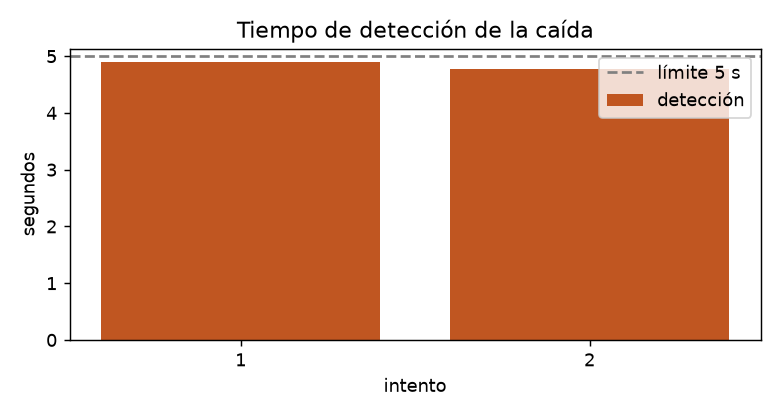
\includegraphics[width=0.7\textwidth]{figuras/tolerancia_fallos.png}
\caption{Tiempo de detección de la caída en cada intento.}
\label{fig:fallos}
\end{figure}

\subsubsection{Disponibilidad del servicio}

Cada 0.5 s se envía una tarea de sondeo mientras nodo-02 falla entre $t = 15$ s y $t = 35$ s.

\begin{table}[htbp]
\centering
\small
\resizebox{\ifdim\width>\linewidth\linewidth\else\width\fi}{!}{%
\begin{tabular}{|c|c|}
\hline
\textbf{Métrica} & \textbf{Valor} \\ \hline
Sondas enviadas & 140 \\ \hline
Completadas & 100.0 \% \\ \hline
Completadas en $\leq$ 3 s & 97.86 \% \\ \hline
\end{tabular}}
\caption{Disponibilidad del servicio durante la falla de un nodo.}
\label{tab:disponibilidad}
\end{table}

\begin{figure}[htbp]
\centering
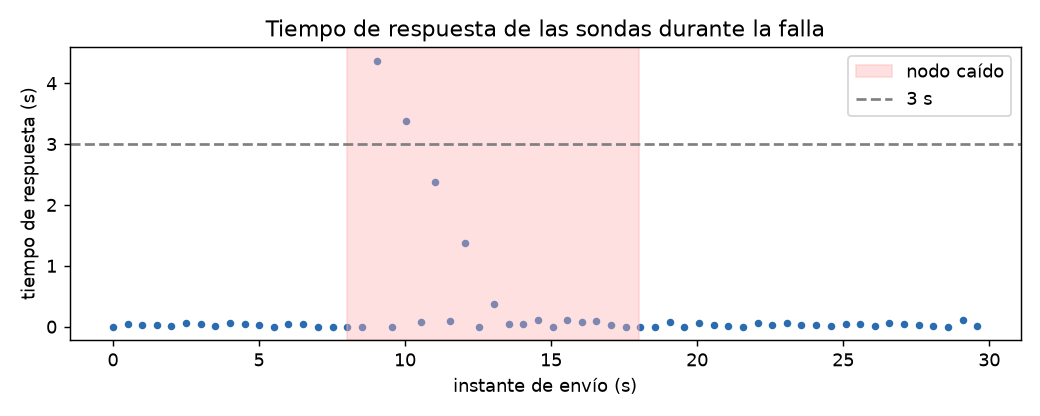
\includegraphics[width=0.9\textwidth]{figuras/disponibilidad.png}
\caption{Tiempo de respuesta de las sondas durante la falla.}
\label{fig:disponibilidad}
\end{figure}

Las sondas enviadas al nodo caído no reciben \texttt{TASK\_ACK}; tras el \emph{timeout} se reasignan a otro nodo y se completan, por eso la disponibilidad es alta pero algunas respuestas tardan alrededor del \emph{timeout} de 5 s.

\subsubsection{Consumo de recursos del nodo coordinador}

\begin{table}[htbp]
\centering
\small
\resizebox{\ifdim\width>\linewidth\linewidth\else\width\fi}{!}{%
\begin{tabular}{|c|c|}
\hline
\textbf{Métrica} & \textbf{Valor} \\ \hline
Mensajes enviados / recibidos & 2124 / 3469 \\ \hline
Tráfico enviado / recibido & 546 KB / 838 KB \\ \hline
Duración & 468 s \\ \hline
Tráfico medio enviado & 1.17 KB/s \\ \hline
Tareas enviadas / completadas / reasignadas / fallidas & 1308 / 1308 / 39 / 0 \\ \hline
\end{tabular}}
\caption{Consumo del nodo que coordinó los experimentos.}
\label{tab:recursos}
\end{table}

\subsubsection{Síntesis de los resultados}

\begin{itemize}
\item \textbf{Descubrimiento:} los nodos se encuentran solos en 0.12 s de media en 5/8 intentos, sin configuración manual.
\item \textbf{Escalabilidad:} con 3 nodos la aceleración fue 1.55$\times$ respecto a un solo nodo.
\item \textbf{Estrategias:} la de menor tiempo total fue Menos cargado.
\item \textbf{Fallos:} la caída se detectó en 4.73 s de media y se completó el 100\,\% de las tareas.
\item \textbf{Disponibilidad:} se completó el 100.0\,\% de las sondas durante la falla de un nodo.
\end{itemize}


\subsection{Pruebas}

El proyecto incluye 66 pruebas automáticas (\texttt{python -m pytest tests}): 42 de las fases anteriores
(planificador, mensajes, reloj de Lamport, tabla de vecinos, detector de fallos y escenarios de
integración con tres nodos reales) y 24 de la Fase 3, que verifican:

\begin{itemize}
\item las seis estrategias y su respeto por los requisitos de la tarea;
\item la normalización robusta (sin amplificar diferencias mínimas) y el ejemplo numérico del diseño;
\item que la suma de los estadísticos de los fragmentos equivale a la regresión sobre todos los datos;
\item la API (\texttt{map} conserva el orden, el requisito de nodos, el cambio de estrategia, \texttt{on\_event});
\item que una alerta llega al registro de todos los nodos;
\item que un nodo caído pasa a \texttt{OFFLINE}, se recupera y que sus tareas se reasignan;
\item que las ranuras limitan la ejecución simultánea y la detección de la subred.
\end{itemize}

\subsection{Qué se puede demostrar en la sustentación}

\begin{itemize}
\item Tres computadores físicos descubriéndose automáticamente en la misma red.
\item El panel web mostrando los tres nodos, sus recursos, la latencia y las tareas en vivo.
\item Las tres aplicaciones: alertas de monitoreo, procesamiento \emph{map-reduce} y regresión
lineal distribuida.
\item La caída de un nodo durante una tarea: alerta crítica, reasignación automática y resultado
correcto.
\item El cambio de estrategia de asignación en caliente y su efecto en el reparto.
\item Las métricas y gráficas de los experimentos.
\end{itemize}

\subsection{Limitaciones}

\begin{itemize}
\item El ancho de banda de cada nodo es un valor declarado, no medido.
\item UDP no garantiza la entrega ni hay retransmisión: la pérdida de un mensaje se maneja con el
\emph{timeout} de la confirmación y la reasignación de la tarea.
\item El nodo que envía una tarea la coordina; si ese nodo cae, pierde el estado de sus tareas, porque
no hay persistencia.
\item La sincronización es un orden lógico de eventos (Lamport); no hay exclusión mutua distribuida.
\item Los \emph{endpoints} de administración no tienen autenticación (uso de laboratorio).
\item Las tareas deben ser lo bastante grandes para amortizar el costo de la comunicación.
\end{itemize}

\subsection{Conclusión de la fase}

Con esta fase se completa ComplexNet API: una red de tres computadores físicos que se descubren solos,
reparten el trabajo con reglas locales, ejecutan aplicaciones de monitoreo, procesamiento y
aprendizaje automático distribuido, detectan fallos y se recuperan sin intervención humana ni
coordinador central. La API permite a otros desarrolladores crear nuevas aplicaciones con pocas líneas,
y la evaluación experimental respalda el comportamiento del sistema en latencia, escalabilidad,
disponibilidad y tolerancia a fallos. Del análisis de las estrategias de asignación resultó una mejora
al modelo original (normalización robusta y término de carga) que evita concentrar las tareas en un
solo nodo.

% Requiere solo el paquete graphicx (ya usado en las secciones anteriores).
% Las tablas y figuras de resultados se generan con
%         python experiments/report.py
% en el archivo fase3_resultados.tex (se incluye al final de esta sección).
% =============================================================================

\section{Descripción del Proyecto -- Fase 3}

\subsection{Objetivo de la fase}

En la Fase 2 se construyó el núcleo de ComplexNet API y se validó con tres nodos en contenedores
Docker dentro de un mismo computador. La Fase 3 convierte ese núcleo en una plataforma utilizable:
se ejecuta sobre \textbf{tres computadores físicos} conectados por una red local, ofrece una
\textbf{API documentada para desarrolladores}, incluye \textbf{tres aplicaciones descentralizadas}
construidas sobre ella, un \textbf{panel de monitoreo} del clúster y una \textbf{evaluación
experimental} de latencia, escalabilidad, disponibilidad, tolerancia a fallos y estrategias de
asignación de tareas.

\subsection{Qué se agregó respecto a la Fase 2}

El núcleo (mensajes JSON sobre UDP, descubrimiento por \emph{beacons}, detección de fallos por
silencio, reasignación de tareas y reloj lógico de Lamport) se mantiene. Lo nuevo es lo siguiente:

\begin{table}[htbp]
\centering
\small
\begin{tabular}{|p{0.2\textwidth}|p{0.33\textwidth}|p{0.33\textwidth}|}
\hline
\textbf{Aspecto} & \textbf{Fase 2} & \textbf{Fase 3} \\ \hline
Despliegue & Tres contenedores Docker en un computador, red virtual & Tres computadores físicos en una red local real \\ \hline
Descubrimiento & \emph{Broadcast} a una subred fija de Docker & Detección automática de la subred y vecinos semilla por IP \\ \hline
Uso del sistema & Script de demostración & API para desarrolladores y manual \\ \hline
Aplicaciones & Una tarea de regresión lineal de ejemplo & Tres aplicaciones descentralizadas \\ \hline
Monitoreo & Terminal y un archivo JSON por nodo & Panel web en vivo con alertas \\ \hline
Planificación & Una función de aptitud $F(i,j)$ & Seis estrategias intercambiables en caliente \\ \hline
Capacidad del nodo & Sin límite de tareas simultáneas & Ranuras de ejecución (\emph{slots}) y cola \\ \hline
Validación & Pruebas funcionales (42) & Pruebas (66) y experimentos con informe \\ \hline
\end{tabular}
\caption{Cambios de la Fase 3 respecto a la Fase 2.}
\label{tab:fase2-fase3}
\end{table}

\subsection{Despliegue en tres computadores}

\paragraph{¿Cómo se conectan los computadores?}
Los tres equipos se conectan a la \textbf{misma red local} (mismo Wi-Fi o router; también sirve el
punto de acceso de un celular). No se usa ningún servidor central ni se necesita internet: cada
nodo envía los mensajes directamente a los demás mediante \textbf{UDP sobre IP}, por el puerto
\texttt{9999}. El panel web usa el puerto \texttt{8000} (TCP) y es solo para observar y administrar.

\begin{table}[htbp]
\centering
\small
\begin{tabular}{|c|c|p{0.5\textwidth}|}
\hline
\textbf{Equipo} & \textbf{Nodo} & \textbf{Qué ejecuta} \\ \hline
Computador 1 & \texttt{nodo-01} & Un nodo, las aplicaciones y los experimentos \\ \hline
Computador 2 & \texttt{nodo-02} & Solo el nodo \\ \hline
Computador 3 & \texttt{nodo-03} & Solo el nodo \\ \hline
\end{tabular}
\caption{Distribución de nodos en los computadores.}
\label{tab:tres-pcs}
\end{table}

\paragraph{Descubrimiento en la red real.}
\begin{enumerate}
\item Cada nodo emite cada 2 s un mensaje \texttt{RESOURCE\_BEACON} por \emph{broadcast} UDP, es decir,
a la dirección que reciben todos los equipos de la subred. El nodo calcula esa dirección a partir de
su propia IP y máscara de red (opción \texttt{--broadcast auto}).
\item El \emph{beacon} informa el identificador del nodo, su IP, su CPU libre, su memoria libre, su ancho
de banda y cuántas tareas tiene en curso.
\item Al recibir el \emph{beacon} de un nodo desconocido, el receptor lo registra en su \texttt{PeerTable}
y le responde con un \emph{beacon} directo. Así, basta con que uno de los dos oiga al otro para que
ambos se descubran.
\item Si la red bloquea el \emph{broadcast} (algunas redes institucionales lo filtran), cada nodo puede
iniciarse con las IP de sus vecinos (\texttt{--peers}) y los mensajes viajan de forma directa. Otra
alternativa es conectar los tres equipos al punto de acceso de un celular.
\end{enumerate}

\paragraph{Mensajes del protocolo.}
Todos los mensajes son JSON con un encabezado (identificador único, emisor, tipo, marca de tiempo y
reloj de Lamport) y una carga útil. El tamaño máximo es de 60 KB, de modo que cada mensaje cabe en un
datagrama UDP.

\begin{table}[htbp]
\centering
\small
\begin{tabular}{|l|p{0.55\textwidth}|}
\hline
\textbf{Mensaje} & \textbf{Función} \\ \hline
\texttt{RESOURCE\_BEACON} & Presencia y recursos del nodo (cada 2 s) \\ \hline
\texttt{PING} / \texttt{PONG} & Medición de la latencia (RTT) entre dos nodos \\ \hline
\texttt{TASK\_SUBMIT} & Envío de una tarea al nodo elegido \\ \hline
\texttt{TASK\_ACK} & Confirmación de recepción de la tarea \\ \hline
\texttt{TASK\_RESULT} & Resultado de la tarea o error \\ \hline
\texttt{ALERT} & Alerta difundida a todos los nodos (Fase 3) \\ \hline
\end{tabular}
\caption{Mensajes intercambiados entre los nodos.}
\label{tab:mensajes}
\end{table}

\paragraph{Puesta en marcha.}
Cada computador ejecuta un único comando, que crea el entorno de Python, instala las dependencias,
abre el puerto en el cortafuegos y arranca el nodo:

\begin{verbatim}
.\scripts\start_node.ps1 -Id nodo-02
\end{verbatim}

\subsection{API para desarrolladores}

La clase \texttt{Node} es la puerta de entrada: oculta el descubrimiento, la planificación, la
comunicación y la recuperación ante fallos. Una aplicación necesita pocas líneas:

\begin{verbatim}
from complexnet import Node, Task

with Node("nodo-01", broadcast_address="auto") as node:
    node.wait_for_peers(2)
    tarea = Task("regresion_lineal", {"n_samples": 10000},
                 requirements={"cpu": 1, "memory": 256})
    resultado = node.submit(tarea)      # el planificador elige el nodo
\end{verbatim}

\begin{table}[htbp]
\centering
\small
\begin{tabular}{|p{0.3\textwidth}|p{0.6\textwidth}|}
\hline
\textbf{Método} & \textbf{Descripción} \\ \hline
\texttt{connect()}, \texttt{disconnect()} & Une el nodo a la red o lo detiene (también como \texttt{with}) \\ \hline
\texttt{wait\_for\_peers(n)} & Espera hasta tener $n$ vecinos activos \\ \hline
\texttt{submit(tarea)} & Envía una tarea y devuelve su resultado (o la tarea, sin esperar) \\ \hline
\texttt{map(nombre, lista)} & Una tarea por elemento; devuelve los resultados en orden \\ \hline
\texttt{map\_tasks(...)} & Igual que \texttt{map}, pero devuelve las tareas con sus tiempos y el nodo ejecutor \\ \hline
\texttt{broadcast(tipo, datos)} & Envía un mensaje a todos los vecinos activos \\ \hline
\texttt{raise\_alert(nivel, texto)} & Registra una alerta y la difunde a toda la red \\ \hline
\texttt{on\_event(funcion)} & Ejecuta una función por cada evento del nodo (fallos, tareas, descubrimiento) \\ \hline
\texttt{set\_strategy(nombre)} & Cambia la estrategia de asignación en caliente \\ \hline
\texttt{simulate\_failure(s)} & Simula una caída del nodo durante $s$ segundos (pruebas) \\ \hline
\texttt{status()} & Estado completo: recursos, vecinos, tareas, alertas y métricas \\ \hline
\end{tabular}
\caption{Métodos principales de la API.}
\label{tab:api}
\end{table}

Una \texttt{Task} lleva un nombre, sus parámetros y requisitos (CPU libre mínima, memoria mínima y,
opcionalmente, una lista de nodos permitidos). Los tipos de tarea disponibles son los siguientes:

\begin{table}[htbp]
\centering
\small
\begin{tabular}{|l|p{0.55\textwidth}|}
\hline
\textbf{Tarea} & \textbf{Descripción} \\ \hline
\texttt{regresion\_lineal} & Regresión lineal completa en un nodo (Fase 2) \\ \hline
\texttt{normal\_equations} & Estadísticos de un fragmento de datos para la regresión distribuida \\ \hline
\texttt{evaluate\_model} & Evaluación de un modelo sobre un fragmento de datos \\ \hline
\texttt{monte\_carlo\_pi} & Estimación de $\pi$ por el método de Monte Carlo \\ \hline
\texttt{word\_count} & Conteo de palabras de un fragmento de texto \\ \hline
\end{tabular}
\caption{Tipos de tarea incluidos.}
\label{tab:tareas}
\end{table}

Agregar una tarea nueva consiste en escribir una función de Python que reciba un diccionario y
devuelva otro, y registrarla en el módulo de ejecutores. La referencia completa está en el manual del
desarrollador (\texttt{docs/api/MANUAL\_DESARROLLADOR.md}).

\subsection{Aplicaciones descentralizadas}

Las tres aplicaciones usan únicamente la API anterior; ninguna depende de un servidor central.

\subsubsection{Aplicación 1: monitoreo distribuido con alertas}

Vigila el clúster con la información que ya circula en los \emph{beacons} y genera alertas que se
\textbf{difunden a todos los nodos}, de modo que cada nodo conserva su propio registro de alertas.

\begin{itemize}
\item \textbf{Crítica:} un nodo pasa a \texttt{OFFLINE}.
\item \textbf{Informativa:} un nodo vuelve a estar \texttt{ONLINE}.
\item \textbf{Advertencia:} CPU libre menor a un umbral, memoria libre menor a un umbral o latencia
mayor a un umbral (configurables).
\end{itemize}

Además guarda una serie de tiempo con la CPU, la memoria y la latencia de cada nodo, y las alertas
aparecen en el panel web.

\subsubsection{Aplicación 2: procesamiento distribuido}

Realiza dos trabajos de tipo \emph{map-reduce} repartidos por la red:

\begin{enumerate}
\item \textbf{Análisis de archivos:} los archivos de texto de una carpeta se parten en fragmentos; cada
nodo cuenta las palabras de su fragmento (\emph{map}) y el nodo coordinador combina los conteos
(\emph{reduce}).
\item \textbf{Cálculo colaborativo:} estimación de $\pi$ por Monte Carlo. Cada nodo lanza puntos al azar
en el cuadrado unidad y cuenta los que caen dentro del círculo; con el total se obtiene
$\pi \approx 4 \cdot \mathrm{dentro} / \mathrm{total}$.
\end{enumerate}

Si un nodo cae durante el trabajo, sus fragmentos se reasignan y el resultado no cambia.

\subsubsection{Aplicación 3: inteligencia artificial distribuida}

Entrena una \textbf{regresión lineal múltiple} repartiendo los datos entre los nodos. La idea es que
la solución de mínimos cuadrados se puede calcular a partir de sumas parciales. Si el conjunto de
datos se divide en fragmentos $(X_k, y_k)$, cada nodo calcula $X_k^{\top}X_k$ y $X_k^{\top}y_k$ de su
fragmento y el coordinador los suma y resuelve:

\begin{equation}
\hat{w} = \Bigl(\sum_k X_k^{\top}X_k\Bigr)^{-1} \sum_k X_k^{\top}y_k
\end{equation}

El resultado es exactamente el de entrenar con todos los datos en un solo equipo. Cada fragmento se
genera dentro del nodo que lo procesa a partir de una semilla, por lo que por la red solo viajan
parámetros pequeños y estadísticos. El modelo se evalúa después en fragmentos nuevos, también
repartidos, calculando el coeficiente de determinación
$R^2 = 1 - \mathrm{SSE}/\mathrm{SST}$. Si un nodo falla durante el entrenamiento, su fragmento se
reasigna a otro y los pesos finales son los mismos.

\begin{table}[htbp]
\centering
\small
\begin{tabular}{|p{0.28\textwidth}|p{0.62\textwidth}|}
\hline
\textbf{Requisito del taller} & \textbf{Cómo se cumple} \\ \hline
Distribución de datos & Fragmentos generados en cada nodo a partir de una semilla \\ \hline
Asignación de recursos & El planificador reparte cada fragmento según CPU, memoria, ancho de banda, latencia, reputación y carga \\ \hline
Información intercambiada & Estadísticos $X_k^{\top}X_k$, $X_k^{\top}y_k$ y sumas de cuadrados, no los datos \\ \hline
Métricas & Error de los pesos, $R^2$, MSE, tiempos y fragmentos por nodo \\ \hline
Tolerancia a fallos & Reasignación automática del fragmento del nodo caído \\ \hline
\end{tabular}
\caption{Aplicación de inteligencia artificial: cumplimiento de los requisitos.}
\label{tab:ia}
\end{table}

\subsection{Estrategias de asignación de tareas}

El planificador de la Fase 2 implementa la función de aptitud del diseño (sección 9):

\begin{equation}
F(i,j) = 0.40\,C' + 0.40\,M' + 0.10\,B' + 0.05\,R - 0.05\,(1 - L')
\end{equation}

donde $C'$, $M'$, $B'$ y $L'$ son la CPU libre, la memoria libre, el ancho de banda y la latencia
(esta última con normalización inversa) normalizados entre los candidatos, y $R$ es la reputación del
nodo. Al probarla en los experimentos se observó un problema: la normalización min-max convierte
diferencias mínimas entre nodos casi idénticos (por ejemplo, 1\,\% de CPU) en diferencias de 0 a 1, y
la función no conoce cuántas tareas tiene ya cada nodo, así que podía enviar todas las tareas al mismo
nodo.

Para resolverlo se agregó la variante \texttt{weighted\_load}, que usa por defecto:

\begin{itemize}
\item \textbf{Normalización robusta:} $x' = (x - \min x) / \max(\max x - \min x,\ \delta)$, donde
$\delta$ es un rango mínimo significativo ($\delta_C = 20$ puntos de CPU libre, $\delta_M = \delta_B = 20\,\%$
del mayor valor y $\delta_L = 5$ ms). Las diferencias de ruido ya no se amplifican.
\item \textbf{Término de carga:} se resta $0.30\,Q'$, donde $Q'$ es el número de tareas en curso del
nodo (incluidas las que el propio coordinador le acaba de enviar) normalizado entre los candidatos; los
pesos de CPU y memoria bajan a 0.25 para que la suma siga siendo 1.
\end{itemize}

\begin{equation}
F_{L}(i,j) = 0.25\,C' + 0.25\,M' + 0.10\,B' + 0.05\,R - 0.05\,(1 - L') - 0.30\,Q'
\end{equation}

Además se implementaron cuatro estrategias de referencia para compararlas:

\begin{table}[htbp]
\centering
\small
\begin{tabular}{|l|p{0.6\textwidth}|}
\hline
\textbf{Estrategia} & \textbf{Criterio} \\ \hline
\texttt{weighted} & $F(i,j)$ del diseño \\ \hline
\texttt{weighted\_load} & $F_L(i,j)$: robusta y con carga (por defecto) \\ \hline
\texttt{least\_loaded} & El nodo con menos tareas en curso \\ \hline
\texttt{lowest\_latency} & El nodo con menor latencia medida \\ \hline
\texttt{round\_robin} & Reparto cíclico entre los candidatos aptos \\ \hline
\texttt{random} & Un candidato apto al azar \\ \hline
\end{tabular}
\caption{Estrategias de asignación implementadas.}
\label{tab:estrategias-lista}
\end{table}

En todas, el conjunto de candidatos se filtra primero con los requisitos de la tarea
($C_i \geq C_{\mathrm{req}}$ y $M_i \geq M_{\mathrm{req}}$) y solo se consideran los nodos activos.

\paragraph{Capacidad de los nodos.}
Cada nodo ejecuta como máximo \texttt{slots} tareas a la vez (2 por defecto); las demás esperan en cola.
Esto modela un computador con CPU limitada y hace que el reparto de carga sea relevante.

\subsection{Panel de monitoreo del clúster}

Cada nodo sirve una página web (\texttt{http://IP-DEL-NODO:8000}) que muestra, en tiempo real, los
nodos del clúster con su estado, CPU, memoria y latencia, la evolución de la latencia, las tareas y sus
resultados, las alertas y el registro de eventos. El mismo servicio expone una API HTTP: consulta del
estado (\texttt{GET /status}, \texttt{GET /events}), envío de tareas (\texttt{POST /tasks}) y
administración para los experimentos (\texttt{POST /admin/fail} para simular una caída remota y
\texttt{POST /admin/strategy} para cambiar la estrategia).

\subsection{Metodología experimental}

Los experimentos se ejecutan con \texttt{experiments/run\_experiments.py} desde el computador 1 y el
informe se genera con \texttt{experiments/report.py} a partir de los archivos CSV resultantes. La carga
de trabajo son tareas de Monte Carlo (intensivas en CPU), y cada medición se repite varias veces para
reportar la media y la desviación estándar. Se evalúan:

\begin{itemize}
\item \textbf{Latencia:} RTT de \texttt{PING}/\texttt{PONG} y tiempo de una tarea mínima.
\item \textbf{Tiempo de descubrimiento:} desde que arranca un nodo nuevo hasta conocer a los demás.
\item \textbf{Escalabilidad:} el mismo lote con 1, 2 y 3 nodos (aceleración) y cargas crecientes.
\item \textbf{Estrategias de asignación:} el mismo lote heterogéneo con las seis estrategias.
\item \textbf{Tolerancia a fallos:} un nodo cae a mitad de un lote y se mide la detección, la
recuperación y el porcentaje de tareas completadas.
\item \textbf{Disponibilidad:} se envía una tarea de sondeo cada 0.5 s mientras un nodo falla.
\end{itemize}

Las fallas se inyectan con el endpoint \texttt{/admin/fail} del nodo víctima, que deja de enviar y
recibir mensajes durante unos segundos, lo que equivale a una caída o a una desconexión de la red.

\subsection{Resultados experimentales}

Las tablas y gráficas de esta sección se generan automáticamente a partir de los datos medidos.

% ARCHIVO GENERADO por experiments/report.py -- no editar a mano.
% Corrida: 20261125-142252

\subsubsection{Entorno}

\begin{table}[htbp]
\centering
\small
\resizebox{\ifdim\width>\linewidth\linewidth\else\width\fi}{!}{%
\begin{tabular}{|c|c|}
\hline
\textbf{Dato} & \textbf{Valor} \\ \hline
Fecha & 2026-11-25 14:22:52 \\ \hline
Entorno & 1 PC (3 procesos en localhost), prueba rapida \\ \hline
Nodos & nodo-01 (127.0.0.1), nodo-03 (127.0.0.1), nodo-02 (127.0.0.1) \\ \hline
Equipo que ejecutó los experimentos & MSI (Windows-11-10.0.26200-SP0) \\ \hline
CPU / RAM de ese equipo & 12 hilos / 15.7 GB \\ \hline
Python & 3.13.7 \\ \hline
Estrategia por defecto & weighted\_load \\ \hline
Tamaño de tarea (puntos Monte Carlo) & 12,000,000 \\ \hline
Modo & rápido (reducido) \\ \hline
\end{tabular}}
\caption{Entorno de la corrida experimental.}
\label{tab:entorno}
\end{table}

\textbf{Nota:} esta corrida se hizo en un solo computador (tres procesos independientes en \texttt{localhost}): los nodos compiten por la misma CPU y la latencia es la de \emph{loopback}. Los experimentos se repiten en los tres computadores físicos para obtener los valores definitivos.

\subsubsection{Latencia de comunicación}

\begin{table}[htbp]
\centering
\small
\resizebox{\ifdim\width>\linewidth\linewidth\else\width\fi}{!}{%
\begin{tabular}{|c|c|c|c|c|c|}
\hline
\textbf{Nodo} & \textbf{Ping medio (ms)} & \textbf{Ping mín (ms)} & \textbf{Ping máx (ms)} & \textbf{Tarea mínima p50 (ms)} & \textbf{Tarea mínima p95 (ms)} \\ \hline
nodo-02 & 0.164 & 0.141 & 0.194 & 1.012 & 1.792 \\ \hline
nodo-03 & 0.344 & 0.32 & 0.376 & 0.915 & 1.415 \\ \hline
\end{tabular}}
\caption{Latencia hacia cada nodo.}
\label{tab:latencia}
\end{table}

\emph{Ping} es el RTT de los mensajes \texttt{PING}/\texttt{PONG} que cada nodo mide a sus vecinos. \emph{Tarea mínima} es el tiempo completo de una tarea \texttt{echo} (asignación, envío, ejecución y respuesta).

\begin{figure}[htbp]
\centering
\includegraphics[width=0.7\textwidth]{images/latencia.png}
\caption{Latencia hacia cada nodo.}
\label{fig:latencia}
\end{figure}

\subsubsection{Tiempo de descubrimiento}

Se arranca un nodo nuevo, sin conocer a nadie, y se mide el tiempo hasta que descubre a todos los demás.

\begin{table}[htbp]
\centering
\small
\resizebox{\ifdim\width>\linewidth\linewidth\else\width\fi}{!}{%
\begin{tabular}{|c|c|c|c|}
\hline
\textbf{Intento} & \textbf{Segundos} & \textbf{Vecinos encontrados} & \textbf{Completo} \\ \hline
1 & 0.101 & 3 & sí \\ \hline
2 & 0.101 & 3 & sí \\ \hline
3 & 0.102 & 3 & sí \\ \hline
\end{tabular}}
\caption{Tiempo de descubrimiento de un nodo nuevo.}
\label{tab:descubrimiento}
\end{table}

Media: \textbf{0.10 s} (mín 0.10 s, máx 0.10 s); descubrimiento completo en 3/3 intentos. El intervalo de los \emph{beacons} es de 2 s, que acota el peor caso.

\subsubsection{Escalabilidad}

\paragraph{Más nodos, misma carga.} Se ejecuta el mismo lote de 12 tareas restringiendo el número de nodos disponibles.

\begin{table}[htbp]
\centering
\small
\resizebox{\ifdim\width>\linewidth\linewidth\else\width\fi}{!}{%
\begin{tabular}{|c|c|c|c|c|}
\hline
\textbf{Nodos} & \textbf{Tiempo total (s)} & \textbf{$\pm$ $\sigma$} & \textbf{Tareas/s} & \textbf{Aceleración} \\ \hline
1 & 1.373 & 0.0 & 8.74 & 1.0$\times$ \\ \hline
2 & 0.821 & 0.0 & 14.62 & 1.67$\times$ \\ \hline
3 & 0.879 & 0.0 & 13.66 & 1.56$\times$ \\ \hline
\end{tabular}}
\caption{Escalabilidad al aumentar el número de nodos.}
\label{tab:escal-nodos}
\end{table}

\begin{figure}[htbp]
\centering
\includegraphics[width=0.9\textwidth]{images/escalabilidad_nodos.png}
\caption{Tiempo total y aceleración según el número de nodos.}
\label{fig:escal-nodos}
\end{figure}

Con 3 nodos la aceleración fue \textbf{1.56$\times$} (ideal: 3$\times$). La diferencia con el ideal se debe a la sobrecarga de coordinación (mensajes, ACK), a que las tareas se reparten en bloques discretos y a las diferencias de capacidad entre equipos.

\paragraph{Incremento progresivo de la carga.}

\begin{table}[htbp]
\centering
\small
\resizebox{\ifdim\width>\linewidth\linewidth\else\width\fi}{!}{%
\begin{tabular}{|c|c|c|c|c|c|c|}
\hline
\textbf{Tareas} & \textbf{Tiempo total (s)} & \textbf{Tareas/s} & \textbf{Latencia media (s)} & \textbf{p95 (s)} & \textbf{Tráfico enviado (KB/s)} & \textbf{CPU usada media (\%)} \\ \hline
4 & 0.371 & 10.77 & 0.252 & 0.371 & 2.55 & nodo-01: 54.2, nodo-03: 17.9, nodo-02: 33.9 \\ \hline
8 & 0.534 & 14.99 & 0.4 & 0.533 & 3.07 & nodo-01: 45.8, nodo-03: 35.6, nodo-02: 35.9 \\ \hline
16 & 1.023 & 15.63 & 0.662 & 0.982 & 4.03 & nodo-01: 44.8, nodo-03: 53.3, nodo-02: 37.9 \\ \hline
\end{tabular}}
\caption{Respuesta del sistema al aumentar la carga.}
\label{tab:escal-carga}
\end{table}

\begin{figure}[htbp]
\centering
\includegraphics[width=0.9\textwidth]{images/carga_progresiva.png}
\caption{Tiempo total y tiempo de respuesta según la carga.}
\label{fig:escal-carga}
\end{figure}

Al multiplicar la carga por 4 (de 4 a 16 tareas) el tiempo total se multiplicó por 2.8 y el rendimiento pasó de 10.77 a 15.63 tareas/s. El tráfico de control fue de 4.03 KB/s con la mayor carga.

\subsubsection{Comparación de estrategias de asignación}

Mismo lote de 18 tareas de tamaño heterogéneo (0.5$\times$, 1$\times$ y 2$\times$) con cada estrategia. \emph{Desbalance} es el coeficiente de variación del número de tareas por nodo (0 = reparto perfecto).

\begin{table}[htbp]
\centering
\small
\resizebox{\ifdim\width>\linewidth\linewidth\else\width\fi}{!}{%
\begin{tabular}{|c|c|c|c|c|c|c|}
\hline
\textbf{Estrategia} & \textbf{Tiempo total (s)} & \textbf{$\pm$ $\sigma$} & \textbf{Latencia media (s)} & \textbf{p95 (s)} & \textbf{Desbalance} & \textbf{Tareas por nodo} \\ \hline
$F(i,j)$ del diseño & 1.804 & 0.0 & 1.01 & 1.797 & 1.414 & nodo-01: 0.0, nodo-02: 18.0, nodo-03: 0.0 \\ \hline
$F(i,j)$ + carga & 1.361 & 0.0 & 0.654 & 1.206 & 0.758 & nodo-01: 11.0, nodo-02: 0.0, nodo-03: 7.0 \\ \hline
Menos cargado & 1.267 & 0.0 & 0.663 & 1.141 & 0.0 & nodo-01: 6.0, nodo-02: 6.0, nodo-03: 6.0 \\ \hline
Menor latencia & 1.563 & 0.0 & 0.876 & 1.492 & 1.414 & nodo-01: 18.0, nodo-02: 0.0, nodo-03: 0.0 \\ \hline
Round-robin & 1.192 & 0.0 & 0.667 & 1.11 & 0.0 & nodo-01: 6.0, nodo-02: 6.0, nodo-03: 6.0 \\ \hline
Aleatoria & 1.145 & 0.0 & 0.639 & 1.021 & 0.36 & nodo-01: 9.0, nodo-02: 4.0, nodo-03: 5.0 \\ \hline
\end{tabular}}
\caption{Comparación de las seis estrategias de asignación.}
\label{tab:estrategias}
\end{table}

\begin{figure}[htbp]
\centering
\includegraphics[width=0.9\textwidth]{images/estrategias.png}
\caption{Tiempo total y equidad del reparto por estrategia.}
\label{fig:estrategias}
\end{figure}

La estrategia con menor tiempo total fue \textbf{Aleatoria} (1.145 s) y la de mayor tiempo \textbf{$F(i,j)$ del diseño} (1.804 s). La función $F(i,j)$ del diseño original tardó 1.804 s con un desbalance de 1.414. Esa función no considera la carga actual y la normalización min-max convierte diferencias mínimas de CPU y memoria entre nodos desocupados en diferencias de 0 a 1, por lo que puede concentrar tareas en pocos nodos. La variante \texttt{weighted\_load} (término de carga y normalización robusta) redujo el tiempo total en 25\,\% y el desbalance de 1.414 a 0.758, conservando el criterio multicriterio.

\emph{Nota: $\sigma = 0$ porque en el modo rápido cada medición se hizo una sola vez.}

\subsubsection{Tolerancia a fallos}

Un nodo cae 2 s después de empezar un lote de tareas (deja de enviar y recibir durante 25 s).

\begin{table}[htbp]
\centering
\small
\resizebox{\ifdim\width>\linewidth\linewidth\else\width\fi}{!}{%
\begin{tabular}{|c|c|c|c|c|c|c|c|c|}
\hline
\textbf{Intento} & \textbf{Nodo caído} & \textbf{Tareas} & \textbf{Completadas} & \textbf{\% completado} & \textbf{Reasignadas} & \textbf{Detección (s)} & \textbf{Recuperación (s)} & \textbf{Tiempo total (s)} \\ \hline
1 & nodo-02 & 12 & 12 & 100.0 & 2 & 4.89 & 1.26 & 8.14 \\ \hline
2 & nodo-03 & 12 & 12 & 100.0 & 2 & 4.77 & 1.18 & 7.95 \\ \hline
\end{tabular}}
\caption{Caída de un nodo durante la ejecución de un lote.}
\label{tab:fallos}
\end{table}

\begin{itemize}
\item Detección de la caída: media \textbf{4.83 s} (requisito: $\leq$ 5 s de silencio; la detección corre cada 0.5 s).
\item Tareas completadas pese a la caída: \textbf{100\,\%} (sin intervención manual).
\item La \emph{recuperación} es el tiempo desde la primera reasignación hasta que la tarea reasignada termina (incluye volver a ejecutarla).
\end{itemize}

\begin{figure}[htbp]
\centering
\includegraphics[width=0.7\textwidth]{images/tolerancia_fallos.png}
\caption{Tiempo de detección de la caída en cada intento.}
\label{fig:fallos}
\end{figure}

\subsubsection{Disponibilidad del servicio}

Cada 0.5 s se envía una tarea de sondeo mientras nodo-02 falla entre $t = 8$ s y $t = 18$ s.

\begin{table}[htbp]
\centering
\small
\resizebox{\ifdim\width>\linewidth\linewidth\else\width\fi}{!}{%
\begin{tabular}{|c|c|}
\hline
\textbf{Métrica} & \textbf{Valor} \\ \hline
Sondas enviadas & 60 \\ \hline
Completadas & 100.0 \% \\ \hline
Completadas en $\leq$ 3 s & 96.67 \% \\ \hline
\end{tabular}}
\caption{Disponibilidad del servicio durante la falla de un nodo.}
\label{tab:disponibilidad}
\end{table}

\begin{figure}[htbp]
\centering
\includegraphics[width=0.9\textwidth]{images/disponibilidad.png}
\caption{Tiempo de respuesta de las sondas durante la falla.}
\label{fig:disponibilidad}
\end{figure}

Las sondas enviadas al nodo caído no reciben \texttt{TASK\_ACK}; tras el \emph{timeout} se reasignan a otro nodo y se completan, por eso la disponibilidad es alta pero algunas respuestas tardan alrededor del \emph{timeout} de 5 s.

\subsubsection{Consumo de recursos del nodo coordinador}

\begin{table}[htbp]
\centering
\small
\resizebox{\ifdim\width>\linewidth\linewidth\else\width\fi}{!}{%
\begin{tabular}{|c|c|}
\hline
\textbf{Métrica} & \textbf{Valor} \\ \hline
Mensajes enviados / recibidos & 598 / 748 \\ \hline
Tráfico enviado / recibido & 153 KB / 174 KB \\ \hline
Duración & 143 s \\ \hline
Tráfico medio enviado & 1.07 KB/s \\ \hline
Tareas enviadas / completadas / reasignadas / fallidas & 286 / 286 / 4 / 0 \\ \hline
\end{tabular}}
\caption{Consumo del nodo que coordinó los experimentos.}
\label{tab:recursos}
\end{table}

\subsubsection{Síntesis de los resultados}

\begin{itemize}
\item \textbf{Descubrimiento:} los nodos se encuentran solos en 0.10 s de media, sin configuración manual.
\item \textbf{Escalabilidad:} con 3 nodos la aceleración fue 1.56$\times$ respecto a un solo nodo.
\item \textbf{Estrategias:} la de menor tiempo total fue Aleatoria.
\item \textbf{Fallos:} la caída se detectó en 4.83 s de media y se completó el 100\,\% de las tareas.
\item \textbf{Disponibilidad:} se completó el 100.0\,\% de las sondas durante la falla de un nodo.
\end{itemize}


\subsection{Pruebas}

El proyecto incluye 66 pruebas automáticas (\texttt{python -m pytest tests}): 42 de las fases anteriores
(planificador, mensajes, reloj de Lamport, tabla de vecinos, detector de fallos y escenarios de
integración con tres nodos reales) y 24 de la Fase 3, que verifican:

\begin{itemize}
\item las seis estrategias y su respeto por los requisitos de la tarea;
\item la normalización robusta (sin amplificar diferencias mínimas) y el ejemplo numérico del diseño;
\item que la suma de los estadísticos de los fragmentos equivale a la regresión sobre todos los datos;
\item la API (\texttt{map} conserva el orden, el requisito de nodos, el cambio de estrategia, \texttt{on\_event});
\item que una alerta llega al registro de todos los nodos;
\item que un nodo caído pasa a \texttt{OFFLINE}, se recupera y que sus tareas se reasignan;
\item que las ranuras limitan la ejecución simultánea y la detección de la subred.
\end{itemize}

\subsection{Qué se puede demostrar en la sustentación}

\begin{itemize}
\item Tres computadores físicos descubriéndose automáticamente en la misma red.
\item El panel web mostrando los tres nodos, sus recursos, la latencia y las tareas en vivo.
\item Las tres aplicaciones: alertas de monitoreo, procesamiento \emph{map-reduce} y regresión
lineal distribuida.
\item La caída de un nodo durante una tarea: alerta crítica, reasignación automática y resultado
correcto.
\item El cambio de estrategia de asignación en caliente y su efecto en el reparto.
\item Las métricas y gráficas de los experimentos.
\end{itemize}

\subsection{Limitaciones}

\begin{itemize}
\item El ancho de banda de cada nodo es un valor declarado, no medido.
\item UDP no garantiza la entrega ni hay retransmisión: la pérdida de un mensaje se maneja con el
\emph{timeout} de la confirmación y la reasignación de la tarea.
\item El nodo que envía una tarea la coordina; si ese nodo cae, pierde el estado de sus tareas, porque
no hay persistencia.
\item La sincronización es un orden lógico de eventos (Lamport); no hay exclusión mutua distribuida.
\item Los \emph{endpoints} de administración no tienen autenticación (uso de laboratorio).
\item Las tareas deben ser lo bastante grandes para amortizar el costo de la comunicación.
\end{itemize}

\subsection{Conclusión de la fase}

Con esta fase se completa ComplexNet API: una red de tres computadores físicos que se descubren solos,
reparten el trabajo con reglas locales, ejecutan aplicaciones de monitoreo, procesamiento y
aprendizaje automático distribuido, detectan fallos y se recuperan sin intervención humana ni
coordinador central. La API permite a otros desarrolladores crear nuevas aplicaciones con pocas líneas,
y la evaluación experimental respalda el comportamiento del sistema en latencia, escalabilidad,
disponibilidad y tolerancia a fallos. Del análisis de las estrategias de asignación resultó una mejora
al modelo original (normalización robusta y término de carga) que evita concentrar las tareas en un
solo nodo.

\end{document}
